\documentclass[,a4paper]{article}
\usepackage{geometry}
\geometry{a4paper,left=35mm,right=35mm, top=25mm, bottom=25mm}
\usepackage[T1]{fontenc}
\usepackage{lmodern}
\usepackage{amssymb,amsmath}
\usepackage{ifxetex,ifluatex}
\usepackage{fixltx2e} % provides \textsubscript
% use microtype if available
\IfFileExists{microtype.sty}{\usepackage{microtype}}{}
\ifnum 0\ifxetex 1\fi\ifluatex 1\fi=0 % if pdftex
  \usepackage[utf8]{inputenc}
\else % if luatex or xelatex
  \usepackage{fontspec}
  \ifxetex
    \usepackage{xltxtra,xunicode}
  \fi
  \defaultfontfeatures{Mapping=tex-text,Scale=MatchLowercase}
  \newcommand{\euro}{€}
\fi
\usepackage{color}
\usepackage{fancyvrb}
\DefineShortVerb[commandchars=\\\{\}]{\|}
\DefineVerbatimEnvironment{Highlighting}{Verbatim}{commandchars=\\\{\}}
% Add ',fontsize=\small' for more characters per line
\newenvironment{Shaded}{}{}
\newcommand{\KeywordTok}[1]{\textcolor[rgb]{0.00,0.44,0.13}{\textbf{{#1}}}}
\newcommand{\DataTypeTok}[1]{\textcolor[rgb]{0.56,0.13,0.00}{{#1}}}
\newcommand{\DecValTok}[1]{\textcolor[rgb]{0.25,0.63,0.44}{{#1}}}
\newcommand{\BaseNTok}[1]{\textcolor[rgb]{0.25,0.63,0.44}{{#1}}}
\newcommand{\FloatTok}[1]{\textcolor[rgb]{0.25,0.63,0.44}{{#1}}}
\newcommand{\CharTok}[1]{\textcolor[rgb]{0.25,0.44,0.63}{{#1}}}
\newcommand{\StringTok}[1]{\textcolor[rgb]{0.25,0.44,0.63}{{#1}}}
\newcommand{\CommentTok}[1]{\textcolor[rgb]{0.38,0.63,0.69}{\textit{{#1}}}}
\newcommand{\OtherTok}[1]{\textcolor[rgb]{0.00,0.44,0.13}{{#1}}}
\newcommand{\AlertTok}[1]{\textcolor[rgb]{1.00,0.00,0.00}{\textbf{{#1}}}}
\newcommand{\FunctionTok}[1]{\textcolor[rgb]{0.02,0.16,0.49}{{#1}}}
\newcommand{\RegionMarkerTok}[1]{{#1}}
\newcommand{\ErrorTok}[1]{\textcolor[rgb]{1.00,0.00,0.00}{\textbf{{#1}}}}
\newcommand{\NormalTok}[1]{{#1}}
% Redefine labelwidth for lists; otherwise, the enumerate package will cause
% markers to extend beyond the left margin.
\makeatletter\AtBeginDocument{%
  \renewcommand{\@listi}
    {\setlength{\labelwidth}{4em}}
}\makeatother
\usepackage{enumerate}
\usepackage{graphicx}
% We will generate all images so they have a width \maxwidth. This means
% that they will get their normal width if they fit onto the page, but
% are scaled down if they would overflow the margins.
\makeatletter
\def\maxwidth{\ifdim\Gin@nat@width>\linewidth\linewidth
\else\Gin@nat@width\fi}
\makeatother
\let\Oldincludegraphics\includegraphics
\renewcommand{\includegraphics}[1]{\Oldincludegraphics[width=\maxwidth]{#1}}
\ifxetex
  \usepackage[setpagesize=false, % page size defined by xetex
              unicode=false, % unicode breaks when used with xetex
              xetex]{hyperref}
\else
  \usepackage[unicode=true]{hyperref}
\fi
\hypersetup{breaklinks=true,
            bookmarks=true,
            pdfauthor={OParl Team - http://oparl.de/},
            pdftitle={OParl Schnittstellen-Spezifikation (Entwurf)},
            colorlinks=true,
            urlcolor=blue,
            linkcolor=magenta,
            pdfborder={0 0 0}}
\setlength{\parindent}{0pt}
\setlength{\parskip}{6pt plus 2pt minus 1pt}
\setlength{\emergencystretch}{3em}  % prevent overfull lines
\setcounter{secnumdepth}{0}

\title{OParl Schnittstellen-Spezifikation (Entwurf)}
\author{OParl Team - http://oparl.de/}
\date{}

\begin{document}
\maketitle

Lizenz: Creative Commons CC-BY-SA

\section{Einleitung}

Dieses Dokument wird bei seiner Fertigstellung die Spezifikation des
OParl Schnittstellen-Standards für parlamentarische Informationssysteme
(Ratsinformationssysteme, RIS) darstellen. Es dient damit als Grundlage
für die Implementierung von OParl-konformen Server- und
Clientanwendungen.

\subsection{Status}

Die Spezifikation befindet sich in Arbeit. Das Dokument enthält
entsprechend viele Ungenauigkeiten und Hinweise auf offene
Fragestellungen.

\subsection{Was ist OParl?}

(Nachfolgend eine Übernahme aus dem bisherigen Abschnitt
``Funktionsumfang der OParl-Schnittstelle''. Der Text sollte deutlich
überarbeitet und erweitert werden.)

Die vorliegende Spezifikation soll eine Webservice-Schnittstelle
definieren, die den anonymen und lesenden Zugriff auf öffentliche
Inhalte aus Parlamentarischen Informationssystemen ermöglicht. Die
Zugriffe erfolgen über das Hypertext Transfer Protocol (HTTP). Daten
werden als JSON oder als JSONP ausgeliefert.

Die Spezifikation wird obligatorische Bestandteile (MUSS) und optionale
Bestandteile (KANN) haben. Der tatsächliche Funktionsumfang kann daher
zwischen den Implementierungen variieren.

\subsection{Zielsetzung von OParl}

\begin{itemize}
\item
  Nutzen für Kommunen, Bürger, politische Parteien
\item
  Nutzen für Anbieter von RIS-Pflegesoftware
\item
  Nutzen für Anbieter von RIS-Darstellungssoftware
\item
  Nutzen für Open Data Initiativen
\item
  Nutzen für die Wissenschaft
\item
  Linked Data erwähnen
\end{itemize}

(Nachstehen der bisherige Textentwurf aus dem Abschnitt ``Motivationen
für den standardisierten Datenzugriff'', der sicherlich deutlich
überarbeitet werden muss.)

Die Gründe, warum Betreiber von parlamentarischen Informationssystemen
den Zugriff darauf über eine standardisierte Schnittstelle ermöglichen
sollten, können vielfältig sein.

Ein zentrales Argument ist die Verpflichtung der Parlamente gegenüber
der Bevölkerung, diese über die Fortschritte der parlamentarischen
Arbeit zu informieren und auf dem Laufenden zu halten. Ein erster
Schritt, der Bevölkerung Einblicke in die Arbeit und Zugriff auf
Dokumente zu gewähren, ist vielerorts in den letzten Jahren durch
Einführung von Ratsinformationssystemen mit anonymem, lesenden Zugriff
über das World Wide Web gemacht worden.

Die damit eingeschlagene Richtung konsequent weiter zu gehen, bedeutet,
die Daten der parlamentarischen Informationssystemen gänzlich offen zu
legen, sofern die Inhalte es erlauben. Es bedeutet, die Daten und
Inhalte so universell weiterverwendbar und so barrierearm wie möglich
anzubieten, dass jegliche weitere Verwendung durch Dritte technisch
möglich ist. Der seit einiger Zeit etablierte Begriff für dieses Prinzip
heißt ``Open Data''.

Das Interesse an parlamentarischen Informationen und an Anwendungen, die
diese nutzbar und auswertbar machen, ist offensichtlich vorhanden. Die
Entwickler der alternativen Ratsinformationssysteme wie Frankfurt
Gestalten{[}14{]}, Offenes Köln{[}15{]} oder der
OpenRuhr:RIS-Instanzen{[}16{]} wissen zu berichten, wie viel Interesse
den Projekten gerade aus Orten entgegen gebracht wird, in denen
derartige Systeme noch nicht verfügbar sind.

Die Anwendungsmöglichkeiten für parlamentarische Informationen, wenn sie
über eine Schnittstelle schnell und einfach abgerufen werden können,
sind vielfältig. Beispiele könnten sein:

\begin{itemize}
\item
  Apps für den Abruf auf mobilen Endgeräten
\item
  Möglichkeiten zur Wiedergabe für Nutzerinnen und Nutzer mit
  Beeinträchtigung des Sehvermögens
\item
  Alternative und erweiterte Suchmöglichkeiten in Inhalten
\item
  Auswertung und Analyse von Themen, Inhalten, Sprache etc.
\item
  Benachrichtigungsfunktionen beim Erscheinen bestimmte Inhalte
\end{itemize}

Die Standardisierung dieses Zugriffs über die Grenzen einzelner Systeme
hinweg erlaubt zudem, diese Entwicklungen grenzüberschreitend zu denken.
Damit steigt nicht nur die potenzielle Nutzerschaft einzelner
Entwicklungen. Auch das Potenzial für Kooperationen zwischen
Anwendungsentwicklern wächst.

Darüber hinaus sind auch Motivationen innerhalb von Organisationen und
Körperschaften erkennbar. So sollen parlamentarische Informationssysteme
vielerorts in verschiedenste Prozesse und heterogene Systemlandschaften
integriert werden. Durch eine einheitliche Schnittstelle bieten sich
effiziente Möglichkeiten zur Integration der Daten in anderen Systeme,
wie beispielsweise Web-Portale.

\subsection{Transparenz und Beteiligung durch Open Data}

\begin{itemize}
\item
  Einführung zu Open Data
\item
  ``10 Principles'' erwähnen
  \url{https://sunlightfoundation.com/policy/documents/ten-open-data-principles/}
\item
  Spürbare Tendenz zu mehr Offenheit
\item
  Open Data ist (nur) zum Teil technisches Problem
\item
  Vier der ``10 Principles'' haben technische Dimension:

  \begin{itemize}
  \item
    \begin{enumerate}[1.]
    \setcounter{enumi}{4}
    \item
      Machine readability
    \end{enumerate}
  \item
    \begin{enumerate}[1.]
    \setcounter{enumi}{5}
    \item
      Non-discrimination
    \end{enumerate}
  \item
    \begin{enumerate}[1.]
    \setcounter{enumi}{6}
    \item
      Use of Commonly Owned Standards
    \end{enumerate}
  \item
    \begin{enumerate}[1.]
    \setcounter{enumi}{8}
    \item
      Permanence
    \end{enumerate}
  \end{itemize}
\item
  Die bloße Bereitstellung einer OParl-konformen API wird weder die
  Einhaltung der technischen Prinzipien, noch der weiteren
  Open-Data-Prinzipien vollständig garantieren. Für echte Transparenz
  bedarft es mehr.
\item
  Viele Bestandteile der Oparl Spezifikation, die einen weitgehend
  barrierearmen Zugang zu Informationen ermöglichen, sind optional.

  \begin{itemize}
  \item
    Beispiel: Volltexte von Dokumenten über die API abrufbar machen
  \end{itemize}
\item
  Andere Bestandteile, die von Interesse wären, sind noch gar nicht von
  OParl abgedeckt. Beispiel: Abstimmungsergebnisse.
\item
  Grund dafür ist, dass sich OParl in einem frühen Stadium befindet und
  primär am Status Quo der parlamentarischen Informationssysteme
  ausgerichtet ist.
\item
  Es liegt also auch weiterhin an den Verwaltungen und Parlamentariern,
  durch einen verantwortungsvollen Umgang mit den Systemen die maximal
  erreichbare Transparenz zu bieten. Das fängt bei Dokumentenformaten an
  (ein PDF mit digitalem Text weist weit weniger Barrieren auf, als ein
  gescannter Brief, der ebenfalls als PDF gespeichert wurde) und hört
  bei der verwendeten Sprache auf.
\end{itemize}

\subsection{Werdegang von OParl 1.0}

Stichpunkte:

\begin{itemize}
\item
  \begin{enumerate}[1.]
  \setcounter{enumi}{16}
  \item
    und 18. November 2012: Die Open Knowledge Foundation Deutschland
    veranstaltet in den Räumen der Heinrich-Böll-Stiftung in Berlin
    einen Workshop für Entwickler von Anwendungen, die einen
    gesellschaftlichen Nutzen bringen sollen. Hier ist VITAKO, die
    Bundes-Arbeitsgemeinschaft der Kommunalen IT-Dienstleister, als
    Sponsor engagiert. Die Geschäftsführerin, Dr.~Marianne Wulff, ist
    persönlich vor Ort. Auch das Projekt Offenes Köln wird in einem
    Vortrag von Marian Steinbach präsentiert. Es kommt zum Austausch
    über die Frage, wie das Prinzip der offenen Ratsinformationen
    effektiv auf weitere Kommunen ausgeweitet werden könnte.
  \end{enumerate}
\item
  \begin{enumerate}[1.]
  \setcounter{enumi}{5}
  \item
    Dezember 2012: Anhörung im Landtag NRW in Düsseldorf zu einer
    Open-Data-Strategie der Landesregierung, wo Jens Klessmann und
    Marian Steinbach als Sachverständige gehört werden. Danach Gespräch
    über Möglichkeiten der Standardisierung offener
    Ratsinformationssysteme.
  \end{enumerate}
\item
  Dezember 2012: Dr.~Marianne Wulff, Jens Klessmann und Marian Steinbach
  beginnen mit der Abstimmung über einen Workshop mit Vertreterinnen und
  Vertretern von Kommunen, kommunalen IT-Dienstleistern, RIS-Anbietern
  und Zivilgesellschaft. Ziel: Die Bereitschaft zur Zusammenarbeit an
  einem gemeinsamen Standard ermitteln. Unterdessen beginnt Marian
  Steinbach mit der Formulierung eines Standard-Entwurfs als
  Diskussionsgrundlage. Der Entwurf wird von Beginn an öffentlich auf
  GitHub.com bereit gestellt.
\item
  \begin{enumerate}[1.]
  \setcounter{enumi}{16}
  \item
    April 2013: Insgesamt 30 Teilnehmer versammeln sich in Köln, um sich
    in einem ersten Treffen über Ziele und Chancen einer
    Standardisierung für offene Ratsinformationen auszutauschen. Als
    Ergebnis wird ein großes Interesse an der weiteren Zusammenarbeit
    auf Basis des vorliegenden Standardentwurfs festgestellt. Als Termin
    für die Fertigstellung der ersten Version der Spezifikation wird der
    30. Juni 2013 festgelegt. Die Initiatoren präsentieren den
    Anwesenden hier erstmals den Namen ``OParl'', der künftig als Marke
    für die Bemühungen der Gruppe stehen soll.
  \end{enumerate}
\item
  \begin{enumerate}[1.]
  \setcounter{enumi}{21}
  \item
    Januar 2014: Nachdem sich die verteilte Zusammenarbeit am
    Standard-Entwurf seit April 2013 als nicht zielführend erwiesen hat,
    laden Jens Klessmann und Marian Steinbach und VITAKO zu einem
    eintägigen OParl-Workshop in Bielefeld ein. Das Ziel ist, die
    Spezifikation so weit wie möglich voran zu treiben und eine gute
    Basis für die baldige Fertigstellung zu legen.
  \end{enumerate}
\end{itemize}

\subsection{Zukunft von OParl}

\begin{itemize}
\item
  Verfeinerung, Lücken schliessen
\item
  Globalisierung
\item
  Erweiterung über die kommunale Ebene hinaus (Land, Bund)
\item
  Vereinheitlichung von Kategorien (Drucksachentypen, Arten von Gremien)
\item
  Erweiterung von Personendaten, z.B. mit Social Media URLs
\item
  Mehr Abfragekriterien
\item
  Suchfunktionen (Volltextsuche)
\item
  Abstimmungsverhalten und maschinenlesbare Protokolle
\item
  Schreibender Zugriff. Auch dazu muss das Rad nicht neu erfunden
  werden. Bestehende bzw. in Entwicklung befindliche Spezifikationen und
  Techniken aus der Linked Data-Welt können verwendet werden. Dazu
  gehören insbesondere die Linked Data Platform des W3C und Hydra.
\end{itemize}

\subsection{Nomenklatur der Spezifikation und Satzkonventionen}

\subsubsection{MÜSSEN, SOLLEN und KÖNNEN bzw. ZWINGEND, EMPFOHLEN und
OPTIONAL}

Dieses Spezifikationsdokument nutzt die Modalverben müssen, können und
sollen in einer Art und Weise, die bestimmte Anforderungen möglichst
unmissverständlich in drei verschiedene Abstufung einteilen lässt. Um
ihre normative Bedeutung zu unterstreichen, werden diese Wörter
grundsätzlich in Großbuchstaben gesetzt.

Diese Konvention ist angelehnt an die Definitionen der Begriffe MUST,
SHOULD und MAY (bzw. MUST NOT, SHOULD NOT und MAY NOT) aus
RFC2119.\footnote{RFC2119 \url{http://tools.ietf.org/html/rfc2119}}

Die Bedeutung im Einzelnen:

\begin{description}
\item[MÜSSEN/MUSS bzw. ZWINGEND:]
Die Erfüllung einer Anforderung, die explizit vom Modalverb MÜSSEN bzw.
MUSS Gebrauch macht, ist zwingend erforderlich.

Die Entsprechung in RFC2119 lautet ``MUST'', ``REQUIRED'' oder
``SHALL''.
\item[NICHT DÜRFEN/DARF NICHT:]
Dieses Stichwort kennzeichnet ein absolutes Verbot.

Die Entsprechung in RFC2119 lautet ``MUST NOT'' oder ``SHALL NOT''.
\item[SOLLEN/SOLL bzw. EMPFOHLEN:]
Mit dem Wort SOLLEN bzw. SOLL sind empfohlene Anforderungen
gekennzeichnet, die von jeder Implementierung erfüllt werden sollen.
Eine Nichterfüllung ist als Nachteil zu verstehen, beispielsweise weil
die Nutzerfreundlichkeit dadurch Einbußen erleidet, und sollte daher
sorgfältig abgewogen werden.

Die Entsprechung in RFC2119 lautet ``SHOULD'' oder ``RECOMMENDED''.
\item[NICHT SOLLEN/SOLL NICHT bzw. NICHT EMPFOHLEN:]
Diese Formulierung wird verwendet, wenn unter gewissen Umständen Gründe
existieren können, die ein bestimmtes Verhalten akzeptabel oder sogar
nützlich erscheinen lassen, jedoch die Auswirkung des Verhaltens vor
einer entsprechenden Implementierung verstanden und abgewogen werden
sollen.

Die Entsprechung in RFC2119 lautet ``SHOULD NOT'' oder ``NOT
RECOMMENDED''.
\item[DÜRFEN/DARF bzw. OPTIONAL:]
Mit dem Wort DÜRFEN bzw. DARF oder OPTIONAL sind optionale Bestandteile
gekennzeichnet. Ein Anbieter könnte sich entscheiden, den entsprechenden
Bestandteil aufgrund besonderer Kundenanforderungen zu unterstützen,
während andere diesen Bestandteil ignorieren könnten. Implementierer von
Clients oder Servern DÜRFEN in solchen Fällen NICHT davon ausgehen, dass
der jeweilige Kommunikationspartner den entsprechenden, optionalen
Anteil unterstützt.

Die Entsprechung in RFC2119 lautet ``MAY'' oder ``OPTIONAL''.
\end{description}

\subsubsection{Besondere Hervorhebungen und Satzkonventionen}

\subsection{Initiatoren}

\subsection{Unterstützer}

\subsection{Autoren}

An diesem Dokument haben mitgewirkt:

Felix Ebert, Jan Erhardt, Jens Klessmann, Andreas Kuckartz, Babett
Schalitz, Marian Steinbach, Thomas Tursics, Jakob Voss

\section{Architektur}

In diesem Abschnitt werden grundlegenden Konzepte, die von OParl
abgedeckt werden, erläutert. Die Erläuterungen sind nicht im engeren
Sinne Teil der Spezifikation, sondern dienen dazu, die
Anwendungsbereiche von OParl und die Funktionen einer OParl-konformen
API verständlicher und konkreter beschreiben zu können.

Da die Architektur auf der generellen Architektur des World Wide Web
(WWW) aufbaut, sind einzelne Konzepte direkt den Begriffen der
Architekturbeschreibung des W3-Konsortiums entlehnt.\footnote{Architecture
  of the World Wide Web, Volume One. \url{http://www.w3.org/TR/webarch/}}

\subsection{Überblick}

\begin{figure}[htbp]
\centering
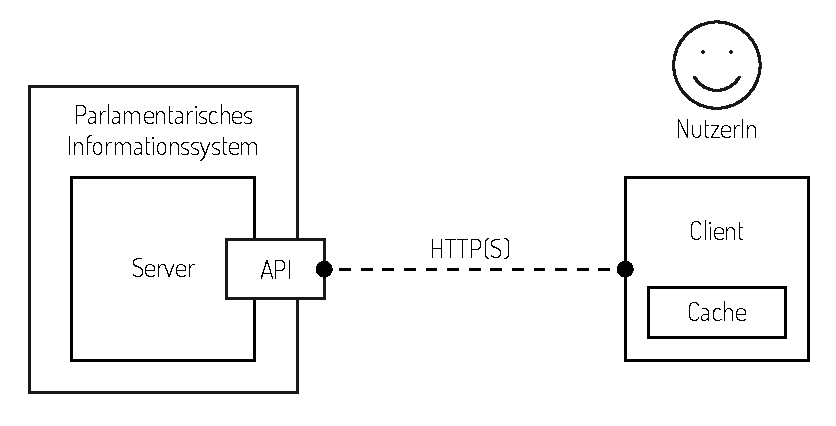
\includegraphics{images/architektur-ueberblick.png}
\caption{Architekturdiagramm}
\end{figure}

\subsection{Parlamentarisches Informationssystem}

Parlamentarische Informationssysteme sind Software-Systeme, die von
verschiedensten Körperschaften eingesetzt werden, um die Zusammenarbeit
von Parlamenten zu organisieren, zu dokumentieren und öffentlich
nachvollziehbar zu machen.

Im kommunalen Umfeld in Deutschland, wo das Parlament je nach Art der
Kommune häufig als Stadtrat oder Gemeinderat bezeichnet wird, hat sich
für diese Art von Informationssystem auch der Begriff
``Ratsinformationssystem'' (kurz ``RIS'') etabliert.

Parlamentarische Informationssysteme sind jedoch nicht auf die kommunale
Ebene begrenzt. Ähnliche Systeme werden auch auf Ebene z.B. von
Landkreisen, Regierungsbezirken und diversen Zweckverbänden eingesetzt.

Diese Systeme unterstützen in der Regel mehrere der folgenden
Funktionen:

\begin{itemize}
\item
  Das Erzeugen, Bearbeiten und Darstellen von Sitzungen und deren
  Tagesordnung
\item
  Das Erzeugen und Abrufen von Sitzungsprotokollen
\item
  Das Erzeugen, Bearbeiten und Anzeigen von Drucksachen
\item
  Das Erzeugen, Bearbeiten und Anzeigen von Gremien und deren
  Mitgliedern
\end{itemize}

Funktionen, die die Eingabe und Bearbeitung von Daten betreffen, sind in
der Regel einem geschlossenen Nutzerkreis vorbehalten. Die Darstellung
und der Abruf von Informationen und Dokumenten hingegen ist in vielen
Fällen für die Öffentlichkeit freigegeben.

Die OParl Spezifikation beschreibt eine Schnittstelle, die den
maschinellen, lesenden Zugriff auf derartige Informationen ermöglicht.

\hyperdef{}{server}{\subsection{Server}\label{server}}

Der Server im Sinne dieser Spezifikation ist ein Software-Dienst, der
auf einem mit dem Internet verbundenen Rechnersystem läuft. Dieser
Dienst ist eine spezielle Form eines WWW- bzw. HTTP(S)-Servers.
Entsprechend beantwortet der Server HTTP-Anfragen, die an ihn auf einem
bestimmten TCP-Port gestellt werden.

Der Server ist als Bestandteil des parlamentarischen Informationssystems
zu verstehen. Der Betrieb des Servers steht damit üblicherweise in der
Verantwortung desjenigen, der das parlamentarischen Informationssystem
betreibt.

Von einem Server, der die OParl-Spezifikation erfüllt, wird erwartet,
dass er bestimmte parlamentarische Informationen in einem bestimmten
Format zur Verfügung stellt und auf bestimmte Anfragen von so genannten
Clients über die OParl API entsprechend dieser Spezifikation reagiert.

\subsection{API}

Der Begriff API steht in diesem Dokument für die
Webservice-Schnittstelle, die der Server anbietet. Die Schnittstelle
basiert auf dem HTTP-Protokoll. Mittels HTTPS ist wahlweise auch die
verschlüsselte Nutzung der API möglich, sofern Server dies unterstützt.

Die API steht im Mittelpunkt dieser Spezifikation. Server und Clients
sind als Kommunikationspartner zu verstehen, die über das Internet als
Kommunikationskanal mit einander kommunizieren können. Die
API-Spezifikation stellt dabei die nötige Grammatik und das Vokabular
bereit, anhand dessen eine sinnvolle Kommunikation erfolgen kann.

\hyperdef{}{client}{\subsection{Client}\label{client}}

Der Begriff ``Client'' steht für eine Software, die über die OParl API
mit dem Server kommuniziert. Da die API auf dem HTTP-Protokoll aufbaut,
handelt es sich bei dem Client um eine spezielle Form eines
HTTP-Clients.

\hyperdef{}{cache}{\subsection{Cache}\label{cache}}

Ein Cache ist ein Speicher, der einem Client dazu dienen kann, von einem
Server abgerufene Informationen längerfristig vorzuhalten. Dies kann
beispielsweise dazu dienen, mehrfache Anfragen der selben Informationen
zu vermeiden, wodurch sowohl Ressourcen auf Seite des Servers geschohnt
als auch die Nutzung von Netzwerkbandbreite reduziert werden kann. Die
Nutzung eines Cache kann auch zur Verbesserung der Nutzerfreundlichkeit
eines Clients beitragen, indem Wartezeiten zur Bereitstellung einer
Ressource verkürzt werden.

\subsection{Nutzerin oder Nutzer}

Mit einer Nutzerin oder einem Nutzer ist in diesem Fall eine natürliche
Person gemeint, die mittels eines OParl-Clients auf parlamentarische
Informationen zugreift.

\subsection{Objekt}

Der Server beantwortet Anfragen eines Clients im Regelfall, indem
bestimmte Objekte ausgegeben werden. Objekte sind im Fall einer
OParl-konformen API JSON-Objekte, die das Schema einhalten, das in der
vorliegenden Spezifikation beaschrieben wird. Antworten des Servers
können einzelne Objekte, Listen von Objekten oder Listen von URLs von
Objekten enthalten.

\section{Nutzungsszenarien}

Die nachfolgenden Nutzungsszenarien dienen dazu, die Architektur und die
Anwendungsmöglichkeiten anhand konkreter Beispiele zu verdeutlichen. Sie
erheben keinen Anspruch auf Vollständigkeit.

\subsubsection{Szenario 1: Mobile Client-Anwendung}

Eine \hyperref[client]{Client}-Anwendung für mobile Endgeräte wie
SmartPhones und Tablets, nachfolgend ``App'' genannt, könnte das Ziel
verfolgen, Nutzern unterwegs sowie abseits vom Desktop-PC bestmöglichen
Lesezugriff auf Dokumente aus Ratsinformationssystemen (RIS) zu bieten.
Die möglichen Kontexte und Nutzungsmotivationen sind vielfältig:

\begin{itemize}
\item
  Teilnehmer einer Sitzung greifen während der Sitzung auf die Einladung
  dieser Sitzung und die zur Tagesordnung der Sitzung gehörenden
  Drucksachen zu, außerdem auf die Protokolle vorheriger Sitzungen.
\item
  Eine Redakteurin der Lokalpresse geht unterwegs die Themen der
  nächsten Sitzungen bestimmter Gremien, für die sie sich besonders
  interessiert, durch.
\item
  Eine Gruppe von Studierenden erkundet zusammen mit ihrem Dozenten die
  lokalpolitischen Aktivitäten des Viertels rund um ihre Hochschule.
  Dazu nutzen sie die GPS-Lokalisierung ihrer Smartphones in Verbindung
  mit den Geodaten, die an vielen Drucksachen des lokalen RIS zu finden
  sind. Direkt vor Ort an einer Baustelle öffnen sie Beschlüsse, Pläne
  und Eingaben aus dem Planfeststellungsverfahren, die dieser Baustelle
  voran gegangen sind.
\end{itemize}

Zur Realisierung derartiger Szenarien können die Fähigkeiten von
OParl-kompatiblen Servern mit den besonderen Eigenschaften der mobilen
Endgeräte verknüpft werden.

Smartphones und Tablets verfügen beispielsweise, je nach Aufenthaltsort,
über sehr unterschiedlich gute Internetanbindung. In einem Büro oder
zuhause können Nutzer über ein WLAN Daten mit hoher Bandbreite
austauschen, in Mobilfunknetzen vor allem außerhalb der Ballungsgebiete
jedoch sinken die Bandbreiten deutlich. Einige Tablets werden sogar ohne
Möglichkeit zur Mobilfunk-Datenübertragung genutzt. In solchen Fällen
kann ein \hyperref[cache]{Cache} auf dem Endgerät dazu dienen, Inhalte
vorzuhalten, die dann auch bei langsamer oder fehlender
Internetverbindung zur Verfügung stehen. Sobald dann wieder eine
Verbindung mit hoher Bandbreite bereit steht, kann die App im
Hintergrund, entweder über die \hyperref[feeds]{Feeds} der OParl API
oder über den einzelnen Abruf von Objekten, die gecachten Inhalte
aktualisieren.

Eine Stärke eines mobilen Clients ist auch die Möglichkeit der
Personalisierung, also der Anpassung auf die Bedürfnisse und Interessen
der Nutzerin oder des Nutzers. Es wäre beispielsweise denkbar, dass eine
Nutzerin die Ratsinformationssysteme, für die sie sich interessiert,
dauerhaft in der App einrichtet und eine Favoritenliste der Gremien, die
ihre bevorzugten Themengebiete behandeln, hinterlegt. Die App könnte
aufgrund dieser Favoritenliste eigenständig über die API nach neuen
Sitzungsterminen, Tagesordnungspunkten, Drucksachen und Dokumente
suchen. Taucht dabei ein neues Objekt auf, wird die Nutzerin darüber
benachrichtigt. Sie kann dann beispielsweise entscheiden, Dokumente
direkt zu öffnen oder für den späteren Offline-Zugriff zu speichern.

Einem derartigen Szenario kommt das Graph-orientierte Datenmodell der
OParl API entgegen. Ausgehend von einer Sitzung eines bestimmten
Gremiums beispielsweise ist es damit einfach möglich, die in Verbindung
stehenden Mitglieder des Gremiums, Teilnehmer der Sitzung,
Tagesordnungspunkte der Sitzung oder Drucksachen zu den
Tagesordnungspunkten und letztlich Dokumente zu Drucksachen und Sitzung
abzurufen.

Für die Nutzer einer mobilen Client-Anwendung könnte es sich als
besonders hilfreich erweisen, wenn Dokumente auf dem Server in
verschiedenen Formaten zur Verfügung gestellt werden. Denn nicht jedes
Endgerät mit kleinem Bildaschirm bietet eine nutzerfreundliche
Möglichkeit, beispielsweise Dokumente im weit verbreiteten PDF-Format
darzustellen. Hier könnte schon der Entwickler der mobilen App
Mechanismen vorsehen, die, sofern vorhanden, besser geeignete Formate
wie z.B. HTML abrufen.

Neben dem kleinen Display kann für einige mobile Endgeräte auch die im
Vergleich zu einem zeitgemäßen Desktop-PC geringere CPU-Leistung eine
Einschränkung darstellen. Solchen Geräten kommt es besonders entgegen,
wenn der Server zu allen Dokumenten auch den reinen Textinhalt abrufbar
macht, der dann beispielsweise für eine Volltextsuche auf dem Endgerät
indexiert werden kann. So wiederum kann auf dem Client eine Suchfunktion
realisiert werden, welche die OParl-API selbst nicht zur Verfügung
stellt.

Eine solche Suchfunktion kann auch über die reine Volltxtsuche hinaus
gehen und über die Suche mittels Text- oder Spracheingabe hinaus gehen.
Denn ein Client könnte von einem \hyperref[server]{Server}-System, das
Drucksachen mit Geoinformationen anbietet, diese abrufen und räumlich
indexieren. Anhand der Position des Geräts, die mittels GPS genau
bestimmt werden kann, könnte so der lokale Cache nach Objekten in der
Umgebung durchsucht werden. Das Ergebnis könnte auf einer Karte
dargestellt oder in einer Ergebnisliste angezeigt werden, die nach
Distanz zum Objekt sortiert werden könnte.

\subsubsection{Szenario 2: Integration in Web-Portal}

Web Portale bieten Nutzern unter anderem die Möglichkeit Anwendungen,
Prozesse und Dienste zu integrieren. Die OParl API stellt einen solchen
Dienst dar und bereitet so den Weg zu angereicherten Portalseiten.
Informationen, die über die API bezogen werden, können in Portlets
organisiert und visualisiert werden. Hierbei können

\begin{enumerate}[1.]
\item
  angemeldete Benutzer
\end{enumerate}

die eingegrenzten Portlet Parameter für den nächsten Besuch zwischen
speichern, während

\begin{enumerate}[1.]
\setcounter{enumi}{1}
\item
  anonyme Benutzer
\end{enumerate}

dies nicht können. In beiden Fällen können Portalnutzer das angezeigte
Portlet nach ihren Bedürfnissen anpassen. Beispielsweise kann ein
solches Portlet eine Liste der Gremien bereitstellen, aus der sich der
Nutzer das interessante Gremium aussucht und aufgrund dieser Auswahl die
Informationen zu den vergangenen / nächsten Sitzungsterminen im Rat,
etwaiger Drucksachen oder Dokumenten erhält und geeignet visualisiert.

Durch eine solche Integration von RIS Informationen in bestehende
Portalsysteme (unter Umständen die kommunale Webseite selbst), ist es
möglich Nutzern zusätzliche Informationen in der bereits gewohnten
Umgebung zu präsentieren und den bestehenden Informationsgehalt und den
Datenbestand aufzuwerten.

\subsubsection{Szenario 3: Meta-Suche}

\subsubsection{Szenario 4: Forschungsprojekt Themen- und Sprachanalyse}

\section{Prinzipien und Funktionen der API}

(In diesem Kapitel werden die Zugriffsmethoden der OParl-konformen
Schnittstelle beschrieben. Hierzu gehören alle chapter-Dateien, deren
Nummerierung mit der Ziffer 6 beginnnt.)

Stichpunkte:

\begin{itemize}
\item
  Grundlage für den Zugriff auf die Schnittstelle ist das Hypertext
  Transfer Protocol (HTTP).
\item
  Optional gzip Encoding und andere Kodierungen, wenn Client und Server
  dies unterstützen
\item
  Das Protokoll ist zustandslos
\item
  Authentifizierung wird nicht benötigt.
\end{itemize}

\hyperdef{}{designprinzipien}{\subsection{Designprinzipien}\label{designprinzipien}}

\subsubsection{Aufbauend auf der gängigen Praxis}

Grundlage für die Erarbeitung der OParl-Spezifikation in der
vorliegenden Version ist eine Analyse der aktuell (2012 bis 2014) in
Deutschland befindlichen Ratsinformationssysteme und ihrer Nutzung.
Erklärtes Ziel für diese Version ist es, mit möglichst geringem
Entwicklungsaufwand auf Seite der Softwareanbieter und Migrationsaufwand
auf Seite der Betreiber zu einer Bereitstellung von parlamentarischen
Informationen über eine OParl API zu gelangen. Hierbei war es von
entscheidender Bedeutung, dass sich die Informationsmodelle der
einschlägigen Softwareprodukte stark ähneln. Für die OParl-Spezifikation
wurde sozusagen ein Datenmodell als ``gemeinsamer Nenner'' auf Basis der
gängigen Praxis beschrieben.

\subsubsection{Verbesserungen gegenüber dem Status Quo wo möglich}

Dort, wo es dem Ziel der einfachen Implementierbarkeit und der einfachen
Migration nicht im Weg steht, erlauben sich die Autoren dieser
Spezifikation, auch Funktionen aufzunehmen, die noch nicht als gängige
Praxis im Bereich der Ratsinformationssysteme bezeichnet werden können
oder welche nur von einzelnen Systemen unterstützt werden. Solche
Funktionen sind dann so integriert, dass sie nicht als zwingende
Anforderung gelten.

Ein Beispiel für eine derartige Funktion ist die Abbildung von Geodaten
im Kontext von Drucksachen (\texttt{oparl:Paper}), um beispielsweise die
Lage eines Bauvorhabens, das in einer Beschlussvorlage behandelt wird,
zu beschreiben. Zwar ist den Autoren nur ein einziges
Ratsinformationssystem\footnote{Das System BoRis der Stadt Bonn
  \url{http://www2.bonn.de/bo_ris/ris_sql/agm_index.asp}} in Deutschland
bekannt, das Geoinformationen - und zwar in Form von Punktdaten, also
einer Kombination aus Längen- und Breitengradangaben - mit Dokumenten
verknüpft. Der Vorteil dieser Funktion ist jedoch anhand zahlreicher
Anwendungsszenarien belegbar. Somit ist der vorliegenden
OParl-Spezifikation die Möglichkeit beschrieben, beliebige
Geodaten-Objekte entsprechend der GeoJSON Spezifikation\footnote{GeoJSON
  \url{http://geojson.org/}} einzubetten. Die Angabe eines einzelnen
Punktes ist dabei nur ein einfacher Sonderfall. Die Spezifikation
erlaubt auch die Kodierung von mehreren Objekten, die Punkte, Linien
oder Polygone repräsentieren können. Vgl. dazu \texttt{oparl:Location}.

Auch die Ausgabe einer Nur-Text-Version im Kontext des Dokuments
(\texttt{oparl:Document}), das den barrierefreien Zugriff auf Inhalte
oder Indexierung für Volltextsuchfunktionen deutlich vereinfacht, ist
eine Möglichkeit, die in der gängigen Praxis noch nicht zu finden ist.
Ebenso die Möglichkeit, Beziehungen zwischen einzelnen Dokumenten
herzustellen, um so von einem Dokument zu anderen Dokumenten mit
identischem Inhalt, aber in anderen technischen Formaten zu verweisen,
etwa von einer ODT-Datei zu einer PDF-Version.

\subsubsection{RESTful}

Die Bezeichnung ``REST'' (für ``Representational State Transfer'') wurde
im Jahr 2000 von Roy Fielding eingeführt\footnote{Fielding, Roy:
  Architectural Styles and the Design of Network-based Software
  Architectures,
  \url{http://www.ics.uci.edu/~fielding/pubs/dissertation/top.htm}}. Die
Definition von Fielding reicht sehr weit und berührt viele Details. In
der Praxis wird der Begriff häufig genutzt, um eine Schnittstelle zu
beschreiben,

\begin{itemize}
\item
  die auf WWW-Technologie aufbaut, insbesondere dem HTTP-Protokoll
\item
  die darauf beruht, dass mittels URL einzelne Ressourcen oder Zustände
  vom Client abgerufen werden können.
\item
  die zustandslos ist. Das bedeutet, die Anfrage eines Clients an den
  Server enthält alle Informationen, die notwendig sind, um die Anfrage
  zu verarbeiten. Auf dem Server wird kein Speicher zur Verfügung
  gestellt, um beispielsweise den Zustand einer Session zu speichern.
\end{itemize}

\subsubsection{Selbstbeschreibungsfähigkeit}

Ausgaben des Servers sollten so beschaffen sein, dass sie für
menschliche NutzerInnen weitgehend selbsterklärend sein können. Dies
betrifft besonders die Benennung von Objekten und Objekteigenschaften.

Um den Kreis der Entwicklerinnen und Entwickler, die mit einer OParl-API
arbeiten können, nicht unnötig einzuschränken, wird hierbei
grundsätzlich auf englischsprachige Begrifflichkeiten gesetzt.

\hyperdef{}{erweiterbarkeit}{\subsubsection{Erweiterbarkeit}\label{erweiterbarkeit}}

Implementierer sollen in der Lage sein, über eine OParl-konforme
Schnittstelle auch solche Informationen auszugeben, die nicht im Rahmen
des OParl-Schemas abgebildet werden können. Dies bedeutet zum einen,
dass ein System Objekttypen unterstützen und ausliefern darf, die nicht
(oder noch nicht) im OParl Schema beschrieben sind. Das bedeutet auch,
dass Objekttypen so um eigene Eigenschaften erweitert werden können, die
nicht im OParl Schema beschrieben sind.

Ein weiterer Aspekt betrifft die Abwärtskompatiblität, also die
Kompatibilität von OParl-Clients mit zukünftigen Schnittstellen. So
können beispielsweise zukünftige Erweiterungen des OParl Schemas, etwa
um neue Objekttypen, genau so durchgeführt werden wie die Erweiterungen
um herstellerspezifische Objekttypen. Ein Client muss diese Anteile
nicht auswerten, sofern sie nicht für die Aufgabe des Clients relevant
sind.

Diese angestrebte Erweiterbarkeit wird durch weitgehend durch das
JSON-LD-Format (TODO: Verweis einfügen) gewährleistet. Es erlaubt die
Verflechtung von Objekttypen-Definitionen aus verschiedenen Schemata.

\subsubsection{Browseability/Verlinkung}

Klassische Webservice-Schnittstellen erfordern von den Entwicklern
vollständige Kenntnis der angebotenen Einstiegspunkte und
Zugriffsmethoden, gepaart mit sämtlichen unterstützten URL-Parametern,
um den vollen Funktionsumfang der Schnittstelle ausschöpfen zu können.

Parlamentarische Informationen sind weitgehend graphartig aufgebaut. Das
bedeutet, dass Objekte häufig mit einer Vielzahl anderer Objekte
verknüpft sind. So ist eine Person beispielsweise Mitglied in mehreren
Gremien, das Gremium hat mehrere Sitzungen abgehalten und zu diesen
Sitzungen gibt es jeweils zahlreiche Drucksachen, die ihrerseits wieder
zahlreiche Dokumente enthalten.

Eine OParl-Schnittstelle gibt jedem einzelnen Objekt eine eindeutige
Adresse, eine URL. Somit kann die Schnittstelle den Verweis von einem
Objekt, beispielsweise einem Gremium, auf ein anderes Objekt, etwa ein
Mitglied des Gremiums, dadurch ausgeben, dass im Kontext des Gremiums
die URL des Mitglieds ausgeben wird. Der Client kann somit ausgehend von
einem bestimmten Objekt die anderen Objekte im System finden, indem er
einfach den angebotenen URLs folgt. Dieses Prinzip wird auch ``Follow
Your Nose'' genannt\footnote{\url{http://patterns.dataincubator.org/book/follow-your-nose.html}}.

\subsection{Zukunftssicherheit}

Wie unter \hyperref[designprinzipien]{Designprinzipien} beschrieben, ist
diese erste Version der OParl-Spezifikation bereits im Wesentlichen von
den Zielen der einfachen Implementierbarkeit und Migration geleitet.

Der Aufwand, den die Betreiber von parlamentarischen
Informationssystemen bei der Bereitstellung von OParl-konformen
Schnittstellen betreiben, soll auch bei der zukünftigen
Weiterentwicklung dieser Spezifikation berücksichtigt werden. Ebenso
soll den Entwicklern von Client-Software zukünftig entgegen kommen, dass
ihre bestehenden Clients auch mit Servern kommunizieren können, die eine
neuere Version der OParl-Spezifikation unterstützen. Dieser Wunsch ist
bereits im Designprinzip \hyperref[erweiterbarkeit]{Erweiterbarkeit}
ausformuliert.

Mit anderen Worten: die Autoren der OParl-Spezifikation beabsichtigen
größtmögliche Zukunftssicherheit und zukünftige Abwärtskompatibilität.
Dieses Ziel wird in Zukunft natürlich abgewägt werden müssen mit dem
Wunsch, sich an Veränderungen und neue Erkenntnisse anzupassen. Eine
Garantie für Zukunftssicherheit kann insofern niemand aussprechen.

\subsection{HTTP und HTTPS}

OParl-Server und -Client kommunizieren miteinander über das
HTTP-Protokoll.

Hierbei SOLL eine verschlüsselte Variante des Protokolls, auch HTTPS
genannt, zum Einsatz kommen, alternativ kann jedoch auch
unverschlüsseltes HTTP verwendet werden. Welche
Verschlüsselungstechnologie im Fall von HTTPS gewählt wird, obliegt dem
Betreiber bzw. Server-Implementierer.

Die Wahl des unverschlüsselten oder verschlüsselten HTTP-Zugriffs hat
Auswirkung auf die im System verwendeten URLs. Wie im Kapitel
\hyperref[urls]{URLs} beschrieben, verfolgt diese Spezifikation die
Festlegung auf genau eine ``kanonische'' URL je Ressource
(URL-Kanonisierung).

Bei unverschlüsseltem Zugriff wird allen URLs, die auf das betreffende
System zeigen, das Schema ``http://'' voran gestellt, beim
verschlüsselten Zugriff stattdessen ``https://''.

Es ist daher ZWINGEND, dass der Server-Betreiber sich zur
URL-Kanonisierung für nur eine von beiden Varianten entscheidet.
Beantwortet das System regulär Anfragen über HTTPS mit der Auslieferung
von Objekten etc., dann MUSS das System bei Anfragen an die
entsprechenden URLs ohne ``https://'' Schema mit einer Weiterleitung
antworten (HTTP Status-Code 301).

Gleiches gilt umgekehrt: beantwortet das System regulär Anfragen über
unverschlüsseltes HTTP, dann MÜSSEN Anfragen auf die entsprechenden URLs
mit ``https://''-Schema mit einer HTTP-Weiterleitung (HTTP Status-Code
301) beantwortet werden.

\hyperdef{}{urls}{\subsection{URLs}\label{urls}}

Den URLs (für ``Uniform Resource Locators'', auch URI für ``Uniform
Resource Identifier'') kommt bei einer OParl-konformen API eine
besondere Bedeutung zu und es werden eine Reihe von Anforderungen an die
Verarbeitung von URLs gestellt.

Die grundsätzliche Funktionsweise von URLs ist in RFC3986
beschrieben\footnote{\url{http://tools.ietf.org/html/rfc3986}}.

Der Aufbau einer beispielhaften URL mit den Bezeichnungen, wie sie in
diesem Dokument Verwendung finden:

\begin{verbatim}
http://refserv.oparl.org/bodies/0/committees/4/members/?skip=234
\__/   \_______________/\_____________________________/ \______/
 |         |                  |                           |
Schema    Host               Pfad                        Query-String
\end{verbatim}

\subsubsection{URL-Kanonisierung}

Absicht ist, dass jedes benannte Objekt, das ein Server über eine
OParl-API anbietet, über genau eine URL identifizierbar und abrufbar
ist. Diese Vereinheitlichung der URL nennen wir Kanonisierung.

Die Kanonisierung ist entscheidend, um erkennen zu können, ob zwei URLs
das selbe Objekt repräsentieren. Sind zwei URLs identisch, sollen
Clients daraus ableiten können, dass diese das selbe Objekt
repräsentieren. Sind zwei URLs unterschiedlich, soll im Umkehrschluss
die Annahme gelten, dass sie zwei verschiedene Objekte repräsentieren.

Der OParl-konforme Server MUSS für jedes benannte Objekt eine kanonische
URL bestimmen können.

Die URL-Kanonisierung betrifft sämtliche Bestandteile der URL.
Entsprechend beginnt diese schon beim \textbf{Schema} und bei der
Entscheidung durch den Betreiber, ob eine OParl-API regulär über HTTP
oder über HTTPS erreichbar sein soll (vgl. {[}HTTP und HTTPS{]}).

Der \textbf{Host}-Teil der URL wird ebenfalls durch die Konfiguration
des Betreibers festgelegt. Obwohl technisch auch die Verwendung einer
IP-Adresse (z.B. ``123.123.123.123'') möglich wäre, SOLL der Betreiber
einen mit Bedacht gewählten Host-Namen einsetzen. Die Vorteile dieser
Lösung gegenüber der Verwendung einer IP-Adresse sind vielfältig:

\begin{itemize}
\item
  NutzerInnen können Host-Namen lesen und interpretieren
\item
  In Kombination mit der richtigen Domain (oder Subdomain) kann der
  Hostname kommunizieren, wer der Betreiber ist.
\item
  Host-Namen können zwischen verschiedenen technischen Systemen (bzw.
  von IP-Adresse zu IP-Adresse) migriert werden, was hilft, die
  Langlebigkeit der URLs zu gewährleisten
\end{itemize}

Eine URL wie

\begin{verbatim}
http://oparl.ratsinformation.stadt-koeln.de/
\end{verbatim}

kommuniziert beispielsweise direkt die Zugehörigkeit zur Stadt Köln als
Betreiber des Systems. Die Bezeichnung ``ratsinformation'' in der
Subdomain zeigt den Zweck des Systems allgemein verständlich an. Der
Host-Name ``oparl.ratsinformation.stadt-koeln.de'' deutet an, dass diese
URL zu einer OParl-Schnittstelle zu diesem System gehört.

Um die Kanonisierung zu gewährleisten, sind vom Betreiber alle
notwendigen Faktoren auszuschließen, die dazu führen können, dass eine
Ressource neben der kanonischen URL noch über andere URLs abrufbar ist.
Diese Faktoren könnten sein:

\begin{itemize}
\item
  Der selbe Server antwortet nicht nur über den kanonischen Host-Namen,
  sondern auch noch über andere Host-Namen. Das könnte zum Beispiel der
  Fall sein, wenn der Host-Name als CNAME für einen anderen Namen
  konfiguriert wurde oder wenn ein DNS A-Record für die IP-Adresse des
  Servers existiert.
\item
  Der Server ist neben dem Host-Namen auch über die IP-Adresse
  erreichbar.
\item
  Zusätzliche Domains, die einen A-Record auf den selben Server besitzen
\end{itemize}

Zu der kanonischen Beispiel-URL
http://oparl.ratsinformation.stadt-koeln.de/ wären eine Reihe von
nicht-kanonischen URL-Varianten denkbar, die technischen auf den selben
Server führen könnten:

\begin{itemize}
\item
  http://83.123.89.102/
\item
  http://oparl.ratsinformation.stadtkoeln.de/
\item
  http://risserv.stadt-koeln.de/
\end{itemize}

Falls es aus technischen Gründen nicht möglich ist, den Zugang auf das
OParl-System über nicht-kanonische URLs zu unterbinden, SOLL eine
entsprechende HTTP-Anfrage mit einer Weiterleitung auf die entsprechende
kanonische URL beantwortet werden. Dabei ist der HTTP-Status-Code 301 zu
verwenden.

Server-Implementierern wird empfohlen, hierfür den Host-Header der
HTTP-Anfrage auszuwerten und mit der konfigurierten Einstellung für den
kanonischen Hostnamen des Systems abzugleichen.

Beim \textbf{Pfad}-Bestandteil der URL MÜSSEN Server-Implementierer
darüber hinaus beachten, dass nur jeweils eine Schreibweise als die
kanonische Schreibweise gelten kann. Dazu gehört auch die Groß- und
Kleinschreibung, die Anzahl von Schrägstrichen als Pfad-Trennzeichen,
die Anzahl von führenden Nullen vor numerischen URL-Bestandteilen und
vieles mehr.

Die Kanonisierung umfasst auch den \textbf{Query-String}-Bestandteil der
URL. Wie auch beim Pfad, gilt hier, dass für jeden Parameter und jeden
Wert im Query-String nur eine kanonische Schreibweise gelten MUSS.

Darüber hinaus SOLL der Server-Implementierer darauf achten, bei
Verwendung von Query-String-Parametern diese in URLs immer nach dem
selben Prinzip zu sortieren. Ein Beispiel: die beiden URLs

\begin{verbatim}
http://oparl.meinris.de/members?body=1&committee=2
http://oparl.meinris.de/members?committee=2&body=1
\end{verbatim}

unterscheiden sich lediglich in der Reihenfolge der
Query-String-Parameter. Da sie jedoch nicht identisch sind, müssen
Clients annehmen, dass beide URLs verschiedene Objekte repräsentieren.
In der Konsequenz kann es zu vermeidbarer Ressourcennutzugn sowohl auf
Client- als auch auf Serverseite kommen.

\subsubsection{Langlebigkeit}

Weiterhin ist es Absicht, dass URLs von Objekten langlebig sind, so dass
sie, wenn sie einmal verbreitet wurden, langfristig zur Abfrage des
dazugehörigen Objekts verwendet werden können.

Um dies zu gewährleisten, wird den \textbf{Betreibern} empfohlen, die
Wahl der Domain, eventuell der Subdomain und letztlich des Host-Namens
sorgfältig auf seine längerfristige Verwendbarkeit abzuwägen.

\textbf{Server-Implementierer} SOLLEN darüber hinaus dafür sorgen, dass
der Pfad-Bestandteil der URLs die Langlebigkeit der URLs unterstützt. Es
gelten die folgenden Empfehlungen, die jedoch keinen Anspruch auf
Vollständigkeit erheben:

\begin{itemize}
\item
  \textbf{Veränderliche Objekt-Eigenschaften nicht als URL-Bestandteil
  nutzen.} In URLs sollten nur Eigenschaften des Objekts aufgenommen
  werden, die keinen Veränderungen unterliegen. Ändert sich
  beispielsweise die Kennung einer Drucksache im Verlauf ihrer Existenz,
  dann scheidet sie für die Bildung der URL aus.
\item
  \textbf{Technische Eigenschaften der Implementierung verbergen.} Ist
  ein OParl-Server beispielsweise in PHP implementiert, sollte dies
  nicht dazu führen, dass im Pfad ein Bestandteil wie ``oparl.php/''
  erscheint. Erfahrungsgemäß überdauern solche URLs nur kurz.
\end{itemize}

Weitere Empfehlungen für langlebige URLs liefern Tim
Berners-Lee\footnote{Berners-Lee, Tim: Cool URIs don't change.
  \url{http://www.w3.org/Provider/Style/URI.html}} sowie die Europäische
Kommission\footnote{Study on persistent URIs, with identification of
  best practices and recommendations on the topic for the MSs and the
  EC. (PDF) \url{http://goo.gl/JaTq6Z}}.

\subsection{Serialisierung mittels JSON-LD und JSONP}

Eine OParl-konforme API gibt Objekte in Form von JSON aus. Die Objekte
werden dabei entsprechend der JSON-LD Spezifikation um Kontexte
erweitert, welche die Selbstbschreibungsfähigkeit der ausgegebenen Daten
verbessert. Auf Anforderung des Clients wird darüber hinaus JSONP
unterstützt.

\subsubsection{JSON}

Die Abkürzung JSON steht für ``JavaScript Object Notation''. Das
JSON-Format ist in RFC4627\footnote{\url{https://tools.ietf.org/html/rfc4627}}
beschrieben. Nachfolgend werden nur die wichtigsten Definitionen
übernommen, um eine Terminologie zur weiteren Verwendung in diesem
Dokument zu etablieren.

Das JSON-Format unterstützt die Ausgabe von vier verschiedenen
primitiven Datentypen:

\begin{itemize}
\item
  \emph{Zeichenkette} (Unicode)
\item
  \emph{Zahl} (sowohl Ganzzahlen als auch Fließkommazahlen)
\item
  \emph{Wahrheitswert} (\texttt{true} oder \texttt{false})
\item
  \emph{Null}
\end{itemize}

Darüber hinaus werden zwei komplexe Datentypen unterstützt:

\begin{itemize}
\item
  \emph{Objekt}: Eine Sammlung von Schlüssel-Wert-Paaren ohne
  Reihenfolge, wobei der Schlüssel eine Zeichenkette sein muss und der
  Wert ein beliebiger Datentyp sein kann.
\item
  \emph{Array}: Eine geordnete Liste mit beliebigen Datentypen.
\end{itemize}

Beispiel eines Objekts in JSON-Notation:

\begin{Shaded}
\begin{Highlighting}[]
\NormalTok{\{}
    \DataTypeTok{"zeichenkette"}\NormalTok{: }\StringTok{"Das ist eine Zeichenkette"}\NormalTok{,}
    \DataTypeTok{"zahl"}\NormalTok{: }\FloatTok{1.23456789}\NormalTok{,}
    \DataTypeTok{"wahrheitswert"}\NormalTok{: }\DecValTok{true}\NormalTok{,}
    \DataTypeTok{"null"}\NormalTok{: }\DecValTok{null}\NormalTok{,}
    \DataTypeTok{"objekt"}\NormalTok{: \{}
        \DataTypeTok{"foo"}\NormalTok{: }\StringTok{"bar"}
    \NormalTok{\},}
    \DataTypeTok{"array"}\NormalTok{: [}\StringTok{"foo"}\NormalTok{, }\StringTok{"bar"}\NormalTok{]}
\NormalTok{\}}
\end{Highlighting}
\end{Shaded}

\subsubsection{JSON-LD}

Das Kürzel LD im Namen ``JSON-LD'' steht für Linked Data. Entsprechend
erweitert die JSON-LD-Spezifikation\footnote{\url{http://www.w3.org/TR/json-ld/}}
das JSON-Format um die Möglichkeit,

\begin{itemize}
\item
  Objekte mit anderen Objekten zu verknüpfen,
\item
  Objekte und Eigenschaften bestimmten Typen zuzuordnen und damit
\item
  Auskunft über die semantische Bedeutung von Objekten und Eigenschaften
  zu geben.
\end{itemize}

Ein Beispiel aus der JSON-LD-Spezifikation illustriert, wie JSON-LD ein
Objekt um zusätzliche semantische Informationen erweitert. Als
Ausgangspunkt dient eine Personenbeschreibung in gewöhnlichem JSON:

\begin{Shaded}
\begin{Highlighting}[]
\NormalTok{\{}
  \DataTypeTok{"name"}\NormalTok{: }\StringTok{"Manu Sporny"}\NormalTok{,}
  \DataTypeTok{"homepage"}\NormalTok{: }\StringTok{"http://manu.sporny.org/"}\NormalTok{,}
  \DataTypeTok{"image"}\NormalTok{: }\StringTok{"http://manu.sporny.org/images/manu.png"}
\NormalTok{\}}
\end{Highlighting}
\end{Shaded}

Als menschlicher Betrachter kann man leicht erkennen, dass die
Eigenschaft \texttt{name} den Namen der Person enthält, dass
\texttt{homepage} die Website der Person sein könnte und dass
\texttt{image} die URL einer Bilddatei der Person sein könnte. Ein
automatisierter Client jedoch, dem die Objekteigenschaften nicht bekannt
sind, kann die Bedeutung dieser Eigenschaften nicht entschlüsseln.

Entsprechend der JSON-LD-Spezifikation kann diese Erläuterung über die
\texttt{@context}-Eigenschaft direkt im selben Objekt, sozusagen als
Unterobjekt, mitgeliefert werden:

\begin{Shaded}
\begin{Highlighting}[]
\NormalTok{\{}
  \DataTypeTok{"@context"}\NormalTok{:}
  \NormalTok{\{}
    \DataTypeTok{"name"}\NormalTok{: }\StringTok{"http://xmlns.com/foaf/0.1/name"}\NormalTok{,}
    \DataTypeTok{"image"}\NormalTok{: \{}
      \DataTypeTok{"@id"}\NormalTok{: }\StringTok{"http://xmlns.com/foaf/0.1/img"}\NormalTok{,}
      \DataTypeTok{"@type"}\NormalTok{: }\StringTok{"@id"}
    \NormalTok{\},}
    \DataTypeTok{"homepage"}\NormalTok{: \{}
      \DataTypeTok{"@id"}\NormalTok{: }\StringTok{"http://xmlns.com/foaf/0.1/homepage"}\NormalTok{,}
      \DataTypeTok{"@type"}\NormalTok{: }\StringTok{"@id"}
    \NormalTok{\}}
  \NormalTok{\},}
  \DataTypeTok{"name"}\NormalTok{: }\StringTok{"Manu Sporny"}\NormalTok{,}
  \DataTypeTok{"homepage"}\NormalTok{: }\StringTok{"http://manu.sporny.org/"}\NormalTok{,}
  \DataTypeTok{"image"}\NormalTok{: }\StringTok{"http://manu.sporny.org/images/manu.png"}
\NormalTok{\}}
\end{Highlighting}
\end{Shaded}

Hier sind die Eigenschaften wie \texttt{image} einer URL wie
http://schema.org/image zugewiesen. Ein Client, der diese URL kennt,
kann daraus folgern, dass über die Objekteigenschaft \texttt{image}
immer die URL eines Bildes zu finden ist. Das Schlüssel-Wert-Paar

\begin{verbatim}
"@type": "@id"
\end{verbatim}

sagt darüber hinaus aus, dass der Wert dieser Eigenschaft die URL eines
anderen Objekts ist\footnote{URLs heißen in der JSON-LD-Spezifikation
  ``IRI'' (für ``Internationalized Resource Identifier''), wir verwenden
  hier jedoch weiterhin die Bezeichnung ``URL''.}. Mittels
\texttt{@type}-Deklaration könnte aber auch beispielsweise eine
Eigenschaft, die im JSON-Sinn eine Zeichenkette ist, als Datum
deklariert werden.

Am obigen Beispiel fällt auf, dass der \texttt{@context}-Teil des
Objects schon mehr Daten umfasst, als die eigentlichen
Objekteigenschaften. Sinnvollerweise kann jedoch der gesamte Inhalt des
\texttt{@context}-Teils in eine externe Ressource ausgelagert werden.
Clients, die eine Vielzahl von gleichartigen Objekten laden und
interpretieren wollen, müssen diese Ressource dann nur einmal laden. Das
Ergebnis könnte so aussehen:

\begin{Shaded}
\begin{Highlighting}[]
\NormalTok{\{}
  \DataTypeTok{"@context"}\NormalTok{: }\StringTok{"http://json-ld.org/contexts/person.jsonld"}\NormalTok{,}
  \DataTypeTok{"name"}\NormalTok{: }\StringTok{"Manu Sporny"}\NormalTok{,}
  \DataTypeTok{"homepage"}\NormalTok{: }\StringTok{"http://manu.sporny.org/"}\NormalTok{,}
  \DataTypeTok{"image"}\NormalTok{: }\StringTok{"http://manu.sporny.org/images/manu.png"}
\NormalTok{\}}
\end{Highlighting}
\end{Shaded}

Die \texttt{@context}-Eigenschaft hat nun als Wert eine URL. Die URL
(hier: http://json-ld.org/contexts/person.jsonld) gibt wiederum in JSON
kodiert die Beschreibung aller möglichen Attribute des Objekts aus.

JSON-LD ermöglicht es auch, für ein Objekt einen Objekttyp zu
kommunizieren. So könnte passend zu unserem Beispiel ausgedrückt werden,
um welche Art von Objekt es sich bei den vorliegenden Daten handelt.
Dazu wird die \texttt{@type}-Eigenschaft verwendet, deren Wert eine URL
ist:

\begin{Shaded}
\begin{Highlighting}[]
\NormalTok{\{}
  \DataTypeTok{"@context"}\NormalTok{: }\StringTok{"http://json-ld.org/contexts/person.jsonld"}\NormalTok{,}
  \DataTypeTok{"@type"}\NormalTok{: }\StringTok{"http://schema.org/Person"}\NormalTok{,}
  \DataTypeTok{"name"}\NormalTok{: }\StringTok{"Manu Sporny"}\NormalTok{,}
  \DataTypeTok{"homepage"}\NormalTok{: }\StringTok{"http://manu.sporny.org/"}\NormalTok{,}
  \DataTypeTok{"image"}\NormalTok{: }\StringTok{"http://manu.sporny.org/images/manu.png"}
\NormalTok{\}}
\end{Highlighting}
\end{Shaded}

Objekte können mehreren Typen zugeordnet sein und damit die Eigenschafen
mehrerer Objekttypen nutzen. Im Fall von OParl kann diese Möglichkeit
genutzt werden, um über die API Eigenschaften auszugeben, die nicht Teil
des OParl-Schemas sind.

\begin{Shaded}
\begin{Highlighting}[]
\NormalTok{\{}
  \DataTypeTok{"@context"}\NormalTok{: \{}
    \DataTypeTok{"oparl"}\NormalTok{: }\StringTok{"http://oparl.org/schema/1.0/"}\NormalTok{,}
    \DataTypeTok{"vendor"}\NormalTok{: }\StringTok{"http://www.vendor.de/oparl/schema/"}
  \NormalTok{\},}
  \DataTypeTok{"@type"}\NormalTok{: [}\StringTok{"oparl:Paper"}\NormalTok{, }\StringTok{"vendor:Drucksache"}\NormalTok{],}
  \DataTypeTok{"title"}\NormalTok{: }\StringTok{"Beschlussvorlage zum Haushalt"}\NormalTok{,}
  \DataTypeTok{"created"}\NormalTok{: }\StringTok{"2013-05-29T14:17:39+02:00"}\NormalTok{,}
  \DataTypeTok{"aktenzeichen"}\NormalTok{: }\StringTok{"ABC123"}
\NormalTok{\}}
\end{Highlighting}
\end{Shaded}

Das Beispiel oben zeigt ein Objekt, das über die
\texttt{@context}-Eigenschaft zwei verschiedene URLs als sogenannte
Vokabulare referenziert. Das eine Vokabular wird durch das Präfix
\texttt{oparl} repräsentiert, das zweite (herstellereigene) durch das
Präfix \texttt{vendor}. Ein JSON-LD-Client setzt Präfix und
Typenbezeichnung letztlich wieder zu einer URL zusammen.

\begin{itemize}
\item
  Aus \texttt{oparl:Paper} wird
  \texttt{http://oparl.org/schema/1.0/Paper}
\item
  Aus \texttt{vendor:Drucksache} wird
  \texttt{http://www.vendor.de/oparl/schema/Drucksache}
\end{itemize}

TODO: Ab hier weiter ausformulieren

Darüber hinaus stellt JSON-LD zusätzliche Anforderungen an JSON-Daten,
die in diesem Abschnitt weiter ausgeführt werden sollen\ldots{}

\begin{itemize}
\item
  Einschränkungen von OParl gegenüber JSON-LD
\item
  Schlüssel in einem JSON-LD-Objekt müssen einzigartig sein.
\item
  Unterscheidung von Groß- und Kleinschreibung
\item
  Benannte Objekte (URL als Schlüssel)
\item
  Anonyme Objekte (Blank Nodes)
\item
  Mime Type application/ld+json
\item
  Kompakte Form mit Verwendung externer @context-URL als
  SOLL-Anforderung
\item
  Verweis auf
  http://www.bmi.bund.de/SharedDocs/Downloads/DE/Themen/OED\_Verwaltung/ModerneVerwaltung/opengovernment.pdf?\_\_blob=publicationFile
\item
  Siehe https://github.com/OParl/specs/issues/77
\item
  Siehe https://github.com/OParl/specs/issues/10
\end{itemize}

\hyperdef{}{jsonp}{\subsubsection{JSONP}\label{jsonp}}

Eine Einschränkung bei der Nutzung von JSON ist das Sicherheitsmodell
von Web-Browsern. Die gängigen Browser erlauben es innerhalb von
Webanwendungen nicht, JSON-Ressourcen von Domains auszulesen, die nicht
der Domain entsprechen, von der die Webanwendung selbst geladen wurde.
AnwendungsentwicklerInnen sind dadurch bei der Implementierung von
Client-Anwendungen eingeschränkt.

Diese Einschränkung gilt nicht fürt JSONP\footnote{TODO: URL zur
  Spezifikation}. Durch JSONP (TODO: Abkürzung erläutern) wird die
JSON-Notation so erweitert, dass der ausgegebene Code ausführbarer
JavaScript-Code wird. Damit wird erreicht, dass der JSON-Code über die
Grenzen von Domains hinweg direkt von Webanwendungen eingebunden werden
kann.

Das folgende Beispiel verdeutlicht den Unterschied zwischen JSON und
JSONP. Zunächst ein einfaches JSON-Beispiel:

\begin{Shaded}
\begin{Highlighting}[]
\NormalTok{\{}
    \DataTypeTok{"foo"}\NormalTok{: }\StringTok{"bar"}
\NormalTok{\}}
\end{Highlighting}
\end{Shaded}

Durch Einbettung in eine sogenannte Callback-Funktion wird daraus JSONP:

\begin{Shaded}
\begin{Highlighting}[]
\ErrorTok{mycallback(}\NormalTok{\{}
    \DataTypeTok{"foo"}\NormalTok{: }\StringTok{"bar"}
\NormalTok{\}}\ErrorTok{)}
\end{Highlighting}
\end{Shaded}

Der Name der Callback-Funktion (im Beispiel ``mycallback'') wird
grundsätzlich bei der Anfrage vom Client bestimmt, und zwar mittels
URL-Parameter.

Für eine OParl-konforme Schnittstelle wird EMPFOHLEN, dass der Server
die JSONP-Ausgabe unterstützt. Die JSONP-Ausgabe MUSS in diesem Fall für
sämtliche Abfragen möglich sein. Eine JSONP-Unterstzung nur für
bestimmte Anfragen ist nicht vorgesehen.

Der URL-Parameter, den Clients zur Aktivierung der JSONP-Ausgabe
verwenden, MUSS \texttt{callback} lauten. Der Wert des
\texttt{callback}-URL-Parameters MUSS vom Server unverändert als
Callback-Funktionsname verwendet werden.

Aus Sicherheitsgründen MUSS der Client den Wert des
\texttt{callback}-Parameters aus einem eingeschränkten Zeichenvorrat
bilden, erlaubt sind ausschließlich die Klein- und Großbuchstaben von a
bis z bzw. A bis Z sowie die Ziffern von 0 bis 9.

Hält sich der Client nicht an diese Einschränkung und wird ein
\texttt{callback}-Parameter mit nicht erlaubten Zeichen verwendet, SOLL
der Server die Anfrage mit einer HTTP XXX (Bad Request) Antwort
bedienen. (TODO: Status Code einfügen oder prüfen, welche HTTP-Antwort
die geeignetste ist.)

\begin{itemize}
\item
  TODO: Spezifikation finden/verlinken. (RFC gibt es nicht)
\item
  https://github.com/OParl/specs/issues/67
\end{itemize}

\subsection{Benannte und anonyme Objekte}

Die JSON-LD-Spezifikation unterscheidet zwischen benannten und anonymen
Objekten. Da die Unterscheidung auch für OParl von Bedeutung ist, wird
sie hier genauer erläutert.

\subsubsection{Benannte Objekte}

Benannte Objekte sind innerhalb einer JSON-LD-Ausgabe diejenigen
Objekte, die durch eine eigene URL identifiziert werden. Als Beispiel
dient ein fiktives Objekt, das ein Client über die URL

\begin{verbatim}
http://refserv.oparl.org/bodies/0/committees/1
\end{verbatim}

abruft:

\begin{Shaded}
\begin{Highlighting}[]
\NormalTok{\{}
    \DataTypeTok{"@id"}\NormalTok{: }\StringTok{"http://refserv.oparl.org/bodies/0/committees/1"}\NormalTok{,}
    \DataTypeTok{"@type"}\NormalTok{: }\StringTok{"http://oparl.org/schema/1.0/committee"}\NormalTok{,}
    \DataTypeTok{"name"}\NormalTok{: }\StringTok{"Hauptausschuss"}
\NormalTok{\}}
\end{Highlighting}
\end{Shaded}

Das Objekt enthält eine Eigenschaft \texttt{@id} mit der URL des Objekts
als Wert.

Das benannte Objekt kann über seine URL sowohl eindeutig identifiziert
als auch direkt abgerufen werden.

\subsubsection{Anonyme Objekte (Blank Nodes)}

Im Gegensatz dazu können Objekte existieren, die keine eigene URL haben.
Ein Beispiel dafür findet sich in der Beratungsfolge einer Drucksache.

Das nachfolgende Beispiel zeigt eine Drucksache, deren Beratungsfolge
über die Eigenschaft \texttt{consultations} kodiert ist.

TODO: Nachstehendes Beispiel und Text dazu auf stimmiges Paper Objekt
umschreiben.

\begin{Shaded}
\begin{Highlighting}[]
\NormalTok{\{}
    \DataTypeTok{"@id"}\NormalTok{: }\StringTok{"http://refserv.oparl.org/bodies/0/papers/456"}\NormalTok{,}
    \DataTypeTok{"@type"}\NormalTok{: }\StringTok{"http://oparl.org/schema/1.0/paper"}\NormalTok{,}
    \DataTypeTok{"title"}\NormalTok{: }\StringTok{"Beschlussvorlage zur Jugendförderung"}\NormalTok{,}
    \DataTypeTok{"consultations"}\NormalTok{: [}
        \NormalTok{\{}
            \DataTypeTok{"@type"}\NormalTok{: }\StringTok{"http://oparl.org/schema/1.0/consultation"}\NormalTok{,}
            \DataTypeTok{"committee"}\NormalTok{: }\StringTok{"http://refserv.oparl.org/bodies/0/committees/1"}\NormalTok{,}
            \DataTypeTok{"meeting"}\NormalTok{: }\StringTok{"http://refserv.oparl.org/bodies/0/committees/1/meetings/123"}\NormalTok{,}
            \DataTypeTok{"agendaitem"}\NormalTok{: }\StringTok{"7.2.4"}\NormalTok{,}
            \DataTypeTok{"authoritative"}\NormalTok{: }\DecValTok{false}
        \NormalTok{\},}
        \NormalTok{\{}
            \ErrorTok{...}
        \NormalTok{\}}
    \NormalTok{]}
\NormalTok{\}}
\end{Highlighting}
\end{Shaded}

Die Eigenschaft \texttt{consultations} ist eine Liste mit einem oder
mehreren Objekten vom Typ \texttt{consultation}. Diese Objekte spiegeln
wieder, in welchen Sitzungen die vorliegende Drucksache beraten wurde
bzw. wird.

Die einzelnen \texttt{consultation}-Objekte haben keine
\texttt{@id}-Eigenschaft, daher handelt es sich dabei um anonyme
Objekte, auch \emph{Blank Nodes} genannt. Diese Objekte können nicht
einzeln, sondern nur im Kontext verbundener Objekte, wie hier im
Beispiel im Kontext einer Drucksache, abgerufen werden.

TODO: Weitere Objekttypen nennen, in denen Blank Nodes vorkommen.

\subsection{Objektlisten}

Über die OParl-API können entweder einzelne Objekte oder Listen von
Objekten abgefragt werden.

\subsubsection{Gezieltes Abfragen von Listen}

Fragt ein Client eine Liste von Objekten an, beispielsweise die Liste
aller Drucksachen in einem System, kann der Server innerhalb bestimmter
Grenzen entscheiden, wie die Ausgabe aussieht.

In der einfachsten Form gibt der Server ein Objekt mit nur einer
Eigenschaft \texttt{items} aus. Der Wert dieser Eigenschaft ist die
\textbf{vollständige Liste} der URLs aller angefragten Objekte.
Beispiel:

\begin{Shaded}
\begin{Highlighting}[]
\NormalTok{\{}
    \DataTypeTok{"items"}\NormalTok{: [}
        \StringTok{"http://refserv.oparl.org/bodies/0/papers/2"}\NormalTok{,}
        \StringTok{"http://refserv.oparl.org/bodies/0/papers/5"}\NormalTok{,}
        \StringTok{"http://refserv.oparl.org/bodies/0/papers/7"}\NormalTok{,}
    \NormalTok{]}
\NormalTok{\}}
\end{Highlighting}
\end{Shaded}

Diese einfachste Form der Antwort eignet sich nur für Listen mit einer
begrenzten Anzahl von Einträgen.

Für längere Listen ist eine Blätterfunktion bzw. Paginierung vorgesehen.
Darunter versteht man den seitenweisen Abruf der Einträge einer Liste,
wobei die Reihenfolge der Liste vom Server festgelegt ist und zwischen
den Seitenabrufen unverändert bleibt.

Listen mit mehr als 100 Einträgen SOLL der Server nur teilweise ausgeben
und dem Client dabei eine \textbf{Paginierung} anbieten, um weitere
Listenteile abzurufen. Dabei wird EMPFOHLEN, die Zahl der jeweils
ausgegebenen Listeneinträge wiederum auf maximal 100 zu begrenzen.

Das nachstehende Beispiel zeigt, wie dem Client die URL zum
``Blättern'', also zum Aufruf der nächsten Listenseite, angeboten wird.

\begin{Shaded}
\begin{Highlighting}[]
\NormalTok{\{}
    \DataTypeTok{"items"}\NormalTok{: [}
        \StringTok{"http://refserv.oparl.org/bodies/0/papers/2"}\NormalTok{,}
        \StringTok{"http://refserv.oparl.org/bodies/0/papers/5"}\NormalTok{,}
        \StringTok{"http://refserv.oparl.org/bodies/0/papers/7"}\NormalTok{,}
    \NormalTok{],}
    \DataTypeTok{"nextpage"}\NormalTok{: }\StringTok{"http://refserv.oparl.org/bodies/0/papers/?skip=7"}\NormalTok{,}
    \DataTypeTok{"count"}\NormalTok{: }\DecValTok{7}
\NormalTok{\}}
\end{Highlighting}
\end{Shaded}

Wie oben zu sehen, enthält das Beispiel-Objekt nun eine zusätzliche
Eigenschaft \texttt{nextpage}. Der Wert dieser Eigenschaft ist eine URL,
die dem Client dazu dient, die weiteren Einträge der Liste abzurufen.

Die Eigenschaft \texttt{count} DARF bei Listen grundsätzlich ausgegeben
werden und SOLL bei mehrseitigen Listen ausgegeben werden. Ihr Wert ist
eine Zahl und gibt an, wie viele Einträge die vollständige Liste
enthält.

Ruft der Client die unter \texttt{nextpage} angegebene URL auf, erhält
er wiederum ein Listenobjekt. Dieses Objekt MUSS, sofern noch immer mehr
Listeneinträge vorhanden sind, als ausgegeben wurden, wiederum die
\texttt{nextpage} Eigenschaft mit einer URL enthalten. Um alle Einträge
einer Liste zu erfassen, folgt der Client also jeweils der URL, die in
der \texttt{nextpage} Eigenschaft angegeben ist.

\begin{figure}[htbp]
\centering
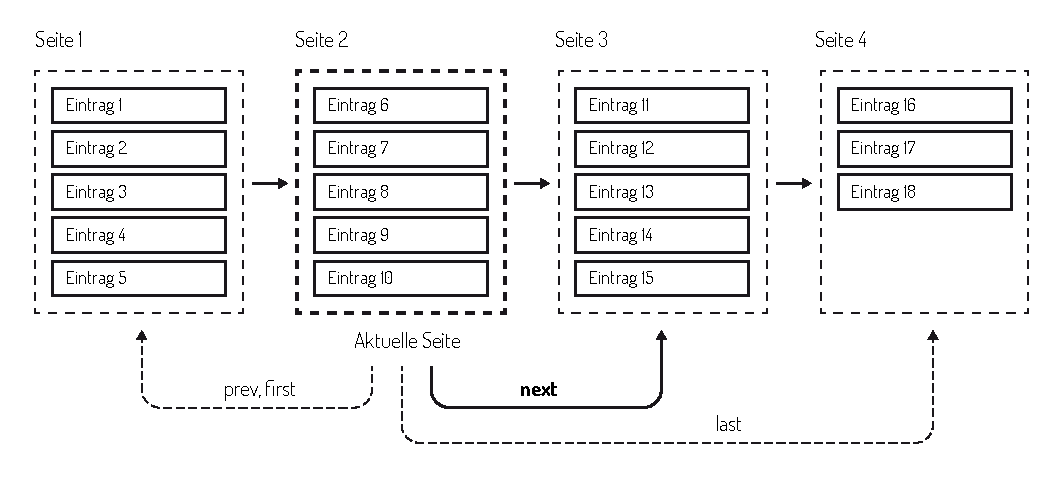
\includegraphics{images/pagination01.png}
\caption{Paginierung: Schematische Darstellung}
\end{figure}

Server-Implementierer entscheiden selbst, wie die \texttt{nextpage}-URL
aufgebaut ist und tragen damit selbst Verantwortung für die
Funktionsweise der Paginierung. Bei der Entscheidung für eine Form der
Implementierung sind weitere Anforderungen zu berücksichtigen:

\begin{itemize}
\item
  Es ist davon auszugehen, dass Clients für den gesamten Abruf aller
  Seiten einer Liste längere Zeit benötigen. In der Zwischenzeit kann
  sich der Inhalt der Liste bereits ändern, etwa durch das Hinzukommen
  neuer Einträge. Die Paginierung ist so zu implementieren, dass sich
  das Hinzukommen oder Entfernen von Einträgen möglichst nicht auf einen
  Client auswirkt, der aktuell die Liste paginiert, um alle Einträge
  abzurufen.
\end{itemize}

Eine ungünstige (unstabile) Form der Implementierung soll hier mit Hilfe
einer SQL-Abfrage illustriert werden. Gegeben sei eine Tabelle
\texttt{example}, die einen numerischen Primärschlüssel \texttt{id}
enthält. Nehmen wir an, die erste Seite der Liste wird mit der Abfrage

\begin{Shaded}
\begin{Highlighting}[]
\KeywordTok{SELECT} \NormalTok{* }\KeywordTok{FROM} \NormalTok{example }\KeywordTok{ORDER} \KeywordTok{BY} \KeywordTok{id} \KeywordTok{LIMIT} \DecValTok{10} \NormalTok{OFFSET }\DecValTok{0}
\end{Highlighting}
\end{Shaded}

abgerufen und würde 10 Datensätze mit den \texttt{id}s 1 bis 10 zurück
liefern. Dann wird die zweite Seite mit der Abfrage

\begin{Shaded}
\begin{Highlighting}[]
\KeywordTok{SELECT} \NormalTok{* }\KeywordTok{FROM} \NormalTok{example }\KeywordTok{ORDER} \KeywordTok{BY} \KeywordTok{id} \KeywordTok{LIMIT} \DecValTok{10} \NormalTok{OFFSET }\DecValTok{10}
\end{Highlighting}
\end{Shaded}

abgerufen. Sofern sich an der Tabelle zwischen den beiden Abfragen
nichts geändert hat, liefert die zweite Abfrage Datensätze mit
\texttt{id} \textgreater{} 10 aus. Sollte zwischen den beiden Abfragen
jedoch beispielsweise der Datensätze mit der \texttt{id} 1 gelöscht
worden sein, liefert die zweite Abfrage Datensätze mit \texttt{id}
\textgreater{} 9. In diesem Fall würde dies nur dazu führen, dass ein
Datensatz (\texttt{id} = 10) zweimal ausgegeben wird. Bei ungünstigeren
Konstellationen wäre auch denkbar, dass eine instabile Paginierung
bewirkt, dass einzelne Datensätze beim Paginieren übergangen werden.

Besser wäre es, bei der Paginierung die Eintragsgrenze, bei der eine
Listenseite beginnen soll, explizit zu benennen. Wurden auf der ersten
Listenseite die Datensätze mit den \texttt{id}s 1 bis 10 ausgegeben, so
könnte der Folgeaufruf, um beim SQL-Beispiel zu bleiben, so aussehen:

\begin{Shaded}
\begin{Highlighting}[]
\KeywordTok{SELECT} \NormalTok{* }\KeywordTok{FROM} \NormalTok{example }\KeywordTok{WHERE} \KeywordTok{id} \NormalTok{> }\DecValTok{10} \KeywordTok{ORDER} \KeywordTok{BY} \KeywordTok{id} \KeywordTok{LIMIT} \DecValTok{10}
\end{Highlighting}
\end{Shaded}

(Hier geht es darum, wie Listen von Objekten ausgegeben werden.

\begin{itemize}
\item
  Einschränkung auf Datumsbereiche
\end{itemize}

Dazu:

\begin{itemize}
\item
  https://github.com/OParl/specs/issues/66
\item
  https://github.com/OParl/specs/issues/30 )
\end{itemize}

\hyperdef{}{feeds}{\subsection{Feeds}\label{feeds}}

\begin{itemize}
\item
  Warum Feeds?
\item
  Möglichst ressourcenschonendes Auffinden neuer und geänderter Objekte
\item
  Cache-Invalidierung, Entfernung von gelöschten/depublizierten Objekten
\item
  https://github.com/OParl/specs/issues/19
\end{itemize}

\subsubsection{Neue Objekte}

\subsubsection{Geänderte Objekte}

\subsubsection{Entfernte Objekte}

\begin{itemize}
\item
  Liste von Objekt-URLs
\end{itemize}

\subsection{Dokumentenabruf}

\begin{itemize}
\item
  HTTP GET Methode MUSS unterstützt werden
\item
  HEAD-Methode MUSS unterstützt werden
\item
  HTTP Last-Modified Header sowie Conditional GET sind zu unterstützen
\end{itemize}

\subsection{Ausnahmebehandlung}

(Diskussion hierzu unter https://github.com/OParl/specs/issues/89)

\subsection{Liste reservierter URL-Parameter}

Die in dieser Liste enthaltenen Zeichenketten haben eine reservierte
Bedeutung und stehen bei Implementierungen eines OParl-Servers nicht
mehr für die freie Verwendung in URLs zur Verfügung.

\begin{description}
\item[callback:]
Mit diesem Parameter wird die JSONP-Ausgabe aktiviert. Mehr dazu im
Abschnitt \hyperref[jsonp]{JSONP}.
\item[startdate:]
Parameter für die Einschränkung einer Abfrage anhand eines Datums bzw.
einer Zeitangabe.
\item[enddate:]
Parameter für die Einschränkung einer Abfrage anhand eines Datums bzw.
einer Zeitangabe.
\end{description}

\begin{itemize}
\item
  (Parameter für Datums-/Zeitbereichsfilter)
\end{itemize}

\section{Schema}

Dieses Kapitel beschreibt das Schema von OParl. Das Schema bildet das
Datzenmodell der OParl-Architektur ab. Es definiert, welche Objekttypen
über eine OParl-API abgerufen werden können und welche Eigenschaften
diese Objekttypen haben dürfen und müssen. Darüber hinaus ist im Schema
auch festgelegt, in welcher Beziehung verschiedene Objekttypen zu
einander stehen.

\subsection{Übergreifende Aspekte}

\subsubsection{null-Werte}

JSON erlaubt es grundsätzlich, dass Eigenschaften den Wert \texttt{null}
haben können. Im Rahmen dieser Spezifikation DARF das jedoch nur bei
Eigenschaften der Fall sein, die als OPTIONAL oder EMPFOHLEN
gekennzeichnet sind. ZWINGENDE Eigenschaften müssen einen Wert ungleich
\texttt{null} besitzen.

\subsubsection{Vererbung der Lizenzbedingung}

\begin{itemize}
\item
  Jedes Objekt KANN die Eigenschaft ``license'' besitzen.
\item
  Die genannte Lizenz bezieht sich auf das jeweilige Objekt und auf
  untergeordnete Objekte, sofern diese keine license-Eigenschaft
  besitzen.
\item
  Dazu muss die Vererbungshierarchie aufgezeigt werden.
\item
  Empfohlene Minimalvariante: Nur eine license-Angabe auf Ebene von
  \texttt{oparl:System}.
\item
  Auf Ebene des \texttt{oparl:Document} bezieht sich die Eigenschaft
  sowohl auf die Metadaten als auch auf das Dokument selbst.
\end{itemize}

\subsubsection{Die Eigenschaften ``created'' und ``last\_modified''}

\subsubsection{Die Eigenschaften ``name'' und ``name\_long''}

\subsubsection{Die Eigenschaft ``description''}

\subsection{OParlSystem (System)}

Der Objekttyp \texttt{oparl:System} bildet grundlegende Informationen
zum parlamentarischen Informationssystem ab. Das Objekt repräsentiert
das technische System, unabhängig von der Frage, welche Körperschaften
auf diesem System vertreten sind.

Auf jedem OParl Server MUSS ein Objekt vom Typ \texttt{oparl:System}
vorgehalten werden. Es DARF nur ein einziges solches Objekt je Server
existieren.

Für Clients ist das \texttt{oparl:System} Objekt ein geeigneter
Einstiegspunkt, um grundlegende Informationen über das Sytem zu bekommen
und die URLs zum Zugriff auf andere Informationen in Erfahrung zu
bringen.

Die URL (IRI) des \texttt{oparl:System} Objekts MUSS per Definition
identisch mit der URL des API-Endpunkts des Servers sein.

\subsubsection{Eigenschaft \texttt{oparl\_version}}

Diese Eigenschaft ist ZWINGEND.

URL der Version der OParl-Spezifikation, die von diesem System
unterstützt wird. So lange es nur die Version 1.0 der
OParl-Spezifikation gibt, MUSS der Wert dieser Eigenschaft
\texttt{http://oparl.org/specs/1.0/} sein.

Sofern zukünftig weitere Versionen der Spezifikation vorliegen, können
Clients damit in Erfahrung bringen, welches Schema, welche Eigenschaften
und Methoden auf Seite des Servers vorausgesetzt werden können.

\subsubsection{Eigenschaft \texttt{bodies}}

Diese Eigenschaft ist ZWINGEND.

Über diese URL sind alle \texttt{oparl:Body} Objekte, also die im System
geführten Körperschaften, als Liste abrufbar.

TODO: Verweis auf \texttt{oparl:Body} einfügen

\subsubsection{Eigenschaft \texttt{name}}

Diese Eigenschaft wird EMPFOHLEN.

Diese Eigenschaft dient dazu, einen nutzerfreundlichen Namen zu
kommunizieren, mit dem NutzerInnen das System wiedererkennen und von
anderen unterscheiden können.

\subsubsection{Eigenschaft \texttt{contact}}

Diese Eigenschaft wird EMPFOHLEN.

Die Eigenschaft dient dazu, NutzerInnen bzw. EntwicklerInnen von Clients
die Kontaktaufnahme mit dem Betreiber des Systems zu ermöglichen. Es
wird EMPFOHLEN, hier die Kontaktdaten eines technischen Ansprechpartners
bzw. einer allgemeinen Kontaktstelle auszugeben, über die Anfragen
verschiedener Art an die richtige Kontaktperson umgeleitet werden
können.

Der Wert dieser Eigenschaft MUSS ein Objekt vom Typ
\texttt{oparl:Contact} sein.

TODO: Verweis auf \texttt{oparl:Contact} einfügen.

\subsubsection{Eigenschaft \texttt{license}}

Diese Eigenschaft wird EMPFOHLEN.

Die Eigenschaft dient dazu, darüber zu informieren, unter welcher Lizenz
die Daten des aktuell angezeigten Objekts stehen. Zur Vererbung dieser
Eigenschaft siehe (TODO: Verweis auf Abschnitt zur Lizenz-Vererbung
einfügen).

Der Wert dieser Eigenschaft sollte nach Möglichkeit eine URL sein, unter
der genau die entsprechende Lizenz abgerufen werden kann.

\subsubsection{Eigenschaft \texttt{new\_objects}}

Diese Eigenschaft ist EMPFOHLEN.

Mit dieser Eigenschaft wird die URL des Feeds für neu hinzugekommene
Objekte ausgegeben.

TODO: Verweis auf Feeds \textgreater{} Neue Objekte

\subsubsection{Eigenschaft \texttt{updated\_objects}}

Diese Eigenschaft ist EMPFOHLEN.

Mit dieser Eigenschaft wird die URL des Feeds für geänderte Objekte
ausgegeben.

TODO: Verweis auf Feeds \textgreater{} Geänderte Objekte

\subsubsection{Eigenschaft \texttt{removed\_objects}}

Diese Eigenschaft ist EMPFOHLEN.

Mit dieser Eigenschaft wird die URL des Feeds für entfernte Objekte
ausgegeben.

TODO: Verweis auf Feeds \textgreater{} Entfernte Objekte

\subsubsection{Eigenschaft \texttt{info}}

Diese Eigenschaft ist OPTIONAL.

Diese Eigenschaft dient dazu, eine zusätzliche URL zu einer WWW-Seite
mit zusätzlichen Informationen zum System anzubieten. So könnten
NutzerInnen beispielsweise auf eine Web-Oberfläche eines
parlamentarischen Informationssystems geführt werden.

\subsubsection{Eigenschaft \texttt{vendor}}

Diese Eigenschaft ist OPTIONAL.

Diese Eigenschaft dient dazu, über eine URL den Hersteller des
Server-Systems zu komunizieren. Die URL sollt nach Möglichkeit zu einer
WWW-Seite mit weiteren Informationen zum Hersteller führen.

\subsubsection{Eigenschaft \texttt{product}}

Diese Eigenschaft ist OPTIONAL.

Diese Eigenschaft dient dazu, über eine URL mitzuteilen, welches
Softwareprodukt das Server-System bereitstellt. Die URL soll nach
Möglichkeit zu einer WWW-Seite mit weiteren Informationen zum Produkt
führen.

\subsubsection{Beispiel}

\begin{Shaded}
\begin{Highlighting}[]
\NormalTok{\{}
    \DataTypeTok{"@id"}\NormalTok{: }\StringTok{"http://refserv.oparl.org/"}\NormalTok{,}
    \DataTypeTok{"@context"}\NormalTok{: }\StringTok{"http://oparl.org/schema/1.0/System"}\NormalTok{,}
    \DataTypeTok{"oparl_version"}\NormalTok{: }\StringTok{"http://oparl.org/specs/1.0/"}\NormalTok{,}
    \DataTypeTok{"name"}\NormalTok{: }\StringTok{"OParl Reference Server"}\NormalTok{,}
    \DataTypeTok{"info"}\NormalTok{: }\StringTok{"https://github.com/OParl/reference-server"}\NormalTok{,}
    \DataTypeTok{"contact"}\NormalTok{: \{}
        \DataTypeTok{"email"}\NormalTok{: }\StringTok{"info@oparl.org"}\NormalTok{,}
        \DataTypeTok{"name"}\NormalTok{: }\StringTok{"Common OParl contact"}
    \NormalTok{\}, }
    \DataTypeTok{"vendor"}\NormalTok{: }\StringTok{"http://oparl.org/"}\NormalTok{,}
    \DataTypeTok{"product"}\NormalTok{: }\StringTok{"https://github.com/OParl/reference-server"}\NormalTok{,}
    \DataTypeTok{"license"}\NormalTok{: }\StringTok{"http://creativecommons.org/licenses/by/4.0/"}\NormalTok{,}
    \DataTypeTok{"bodies"}\NormalTok{: }\StringTok{"http://refserv.oparl.org/bodies/"}\NormalTok{,}
    \DataTypeTok{"new_objects"}\NormalTok{: }\StringTok{"http://refserv.oparl.org/feeds/new/"}\NormalTok{,}
    \DataTypeTok{"updated_objects"}\NormalTok{: }\StringTok{"http://refserv.oparl.org/feeds/updated/"}\NormalTok{,}
    \DataTypeTok{"removed_objects"}\NormalTok{: }\StringTok{"http://refserv.oparl.org/feeds/removed/"}
\NormalTok{\}}
\end{Highlighting}
\end{Shaded}

\subsection{oparl:Body (Körperschaft)}

Dieser Objekttyp erlaubt es, eine Körperschaft abzbilden. Eine
Körperschaft kann beispielsweise eine Gemeinde, ein Landkreis oder ein
Zweckverband sein.

Von einem funktionsfähigen Server wird erwartet, dass er mindestens ein
Objekt vom Typ \texttt{oparl:Body} bereit hält. Teilen sich mehrere
Körperschaften das selbe technische System, können auf demselben Server
auch mehrere Objekte vom Typ \texttt{oparl:Body} beherbergt werden.

Über die Zuordnung zu einem bestimmten \texttt{oparl:Body} Objekt zeigen
andere Objekte, wie beispielsweise Gremien oder Drucksachen, ihre
Zugehörigkeit zu einer bestimmten Körperschaft an.

\begin{figure}[htbp]
\centering
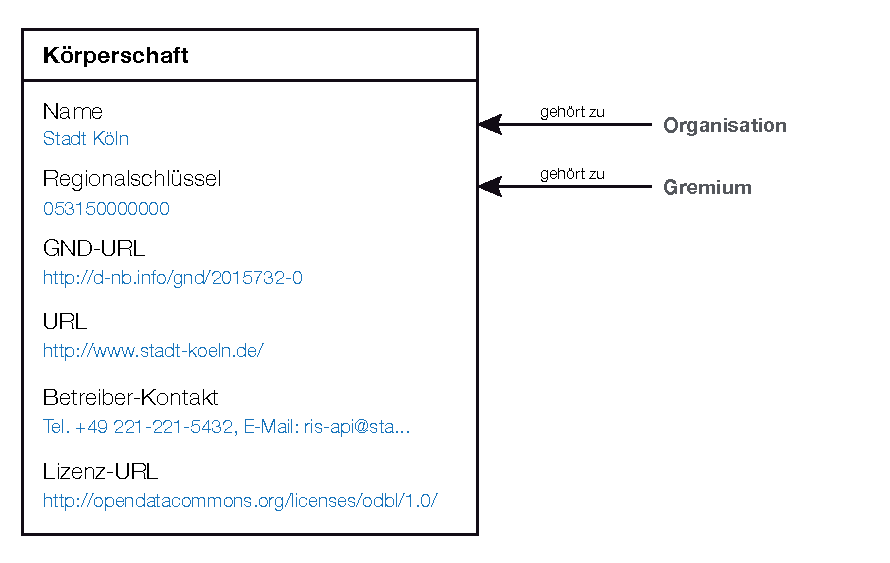
\includegraphics{images/datenmodell_koerperschaft.png}
\caption{Objekttyp oparl:Body}
\end{figure}

Es werden mehrere Eigenschaften angeboten, die dazu dienen, die real
existierende Körperschaft, die von einem \texttt{oparl:Body} Objekt
repräsentiert wird, programmatisch auslesbar zu machen zu können.
Insbesondere sind hier die Eigenschaften \texttt{url}, \texttt{rgs} und
\texttt{gnd\_url} zu nennen.

\subsubsection{Eigenschaft \texttt{system}}

Diese Eigenschaft ist ZWINGEND.

Mit dieser Eigenschaft wird das Objekt dem übergeordneten
\texttt{oparl:System} Objekt zugeordnet. Wert MUSS der IRI des
\texttt{oparl:System} Objekts sein.

\subsubsection{Eigenschaft \texttt{name}}

Diese Eigenschaft ist ZWINGEND. Sie transportiert den gebräuchlichen
Namen der Körperschaft.

\subsubsection{Eigenschaft \texttt{name\_long}}

Diese Eigenschaft ist OPTIONAL und kann bei Bedarf dazu verwendet
werden, eine längere Form des Namens der Körperschaft wieder zu geben,
sofern dieser für die Eigenschaft \texttt{name} zu lang ist.

\subsubsection{Eigenschaft \texttt{url}}

Diese Eigenschaft ist EMPFOHLEN.

Mit dieser Eigenschaft SOLL die URL der offiziellen Website der
Körperschaft ausgegeben werden.

TODO: Beschreibung

\subsubsection{Eigenschaft \texttt{rgs}}

Diese Eigenschaft ist EMPFOHLEN.

Handelt es sich bei der Körperschaft um eine Gebietskörperschaft
(Landkreis, Kommune etc.) in Deutschland, SOLL für die eindeutige
Identifizierung der amtliche Regionalschlüssel verwendet
werden.\footnote{Regionalschlüssel können im
  \href{https://www.destatis.de/DE/ZahlenFakten/LaenderRegionen/Regionales/Gemeindeverzeichnis/Gemeindeverzeichnis.html}{Gemeindeverzeichnis
  (GV-ISys) des Statistischen Bundesamtes} eingesehen werden} Dieser ist
grundsätzlich zwölfstellig.

\subsubsection{Eigenschaft \texttt{gnd\_url}}

Diese Eigenschaft ist EMPFOHLEN.

Sofern die Körperschaft in der GND\footnote{Gemeinsame Normdatei
  \url{http://www.dnb.de/gnd}} vertreten ist, SOLL diese Eigenschaft als
Wert die URL des Eintrags in der GND enthalten.

\subsubsection{Eigenschaft \texttt{contact}}

Diese Eigenschaft ist EMPFOHLEN.

Über diese Eigenschafte SOLLEN Kontaktinformationen zu einer Stelle
bereit gestellt werden, die die inhaltliche Verantwortung für sämtliche
zu dieser Körperschaft gehörenden Inhalte im System trägt. Besonders
wichtig ist diese Angabe, wenn auf einem System mehrere Körperschaften
vertreten sind und damit auf der Ebene des \texttt{oparl:System} Objekts
ein rein technischer Kontakt ausgegeben wird, der nicht für inhaltliche
Fragestellungen im Zuständigkeitsbereich der jeweiligen Körperschaften
kontaktiert werden sollte.

\subsubsection{Eigenschaft \texttt{papers}}

Diese Eigenschaft ist ZWINGEND.

Wert dieser Eigenschaft ist die URL der API zum Aufruf einer Liste der
Drucksachen (Objekte vom Typ \texttt{oparl:Paper}) für diese
Körperschaft.

\subsubsection{Eigenschaft \texttt{people}}

Diese Eigenschaft ist ZWINGEND.

Wert dieser Eigenschaft ist die URL der API zum Aufruf einer Liste der
Personen (Objekte vom Typ \texttt{oparl:Person}) für diese Körperschaft.

\subsubsection{Eigenschaft \texttt{meetings}}

Diese Eigenschaft ist ZWINGEND.

Wert dieser Eigenschaft ist die URL der API zum Aufruf einer Liste der
Sitzungen (Objekte vom Typ \texttt{oparl:Meeting}) für diese
Körperschaft.

\subsubsection{Eigenschaft \texttt{committees}}

Diese Eigenschaft ist ZWINGEND.

Wert dieser Eigenschaft ist die URL der API zum Aufruf einer Liste der
Gremien (Objekte vom Typ \texttt{oparl:Committee}) für diese
Körperschaft.

\subsubsection{Beispiel}

\begin{Shaded}
\begin{Highlighting}[]
\NormalTok{\{}
    \DataTypeTok{"@id"}\NormalTok{: }\StringTok{"http://refserv.oparl.org/bodies/0"}\NormalTok{,}
    \DataTypeTok{"@context"}\NormalTok{: }\StringTok{"http://oparl.org/schema/1.0/Body"}\NormalTok{,}
    \DataTypeTok{"committees"}\NormalTok{: }\StringTok{"http://refserv.oparl.org/bodies/0/committees/"}\NormalTok{,}
    \DataTypeTok{"contact"}\NormalTok{: \{}
        \DataTypeTok{"email"}\NormalTok{: }\StringTok{"ris@stadt-koeln.de"}\NormalTok{,}
        \DataTypeTok{"name"}\NormalTok{: }\StringTok{"RIS-Betreuung"}
    \NormalTok{\}, }
    \DataTypeTok{"created"}\NormalTok{: }\StringTok{"2014-01-08T14:28:31.568+0100"}\NormalTok{,}
    \DataTypeTok{"gnd_url"}\NormalTok{: }\StringTok{"http://d-nb.info/gnd/2015732-0"}\NormalTok{,}
    \DataTypeTok{"last_modified"}\NormalTok{: }\StringTok{"2014-01-08T14:28:31.568+0100"}\NormalTok{,}
    \DataTypeTok{"meetings"}\NormalTok{: }\StringTok{"http://refserv.oparl.org/bodies/0/meetings/"}\NormalTok{,}
    \DataTypeTok{"name"}\NormalTok{: }\StringTok{"Stadt K\textbackslash{}u00f6ln"}\NormalTok{,}
    \DataTypeTok{"name_long"}\NormalTok{: }\StringTok{"Stadt K\textbackslash{}u00f6ln, kreisfreie Stadt"}\NormalTok{,}
    \DataTypeTok{"organisations"}\NormalTok{: }\StringTok{"http://refserv.oparl.org/bodies/0/organisations/"}\NormalTok{,}
    \DataTypeTok{"papers"}\NormalTok{: }\StringTok{"http://refserv.oparl.org/bodies/0/papers/"}\NormalTok{,}
    \DataTypeTok{"people"}\NormalTok{: }\StringTok{"http://refserv.oparl.org/bodies/0/people/"}\NormalTok{,}
    \DataTypeTok{"rgs"}\NormalTok{: }\StringTok{"053150000000"}\NormalTok{,}
    \DataTypeTok{"system"}\NormalTok{: }\StringTok{"http://refserv.oparl.org/"}\NormalTok{,}
    \DataTypeTok{"url"}\NormalTok{: }\StringTok{"http://www.stadt-koeln.de/"}
\NormalTok{\}}
\end{Highlighting}
\end{Shaded}

\subsection{oparl:Committee (Gremium)}

Das Gremium ist ein Personenkreis, üblicherweise von gewählten und/oder
ernannten Mitgliedern. Beispiele hierfür sind der Stadtrat, Kreisrat,
Gemeinderat, Ausschüsse und Bezirksvertretungen. Gremien halten
Sitzungen ab, zu denen die Gremien-Mitglieder eingeladen werden.

\begin{figure}[htbp]
\centering
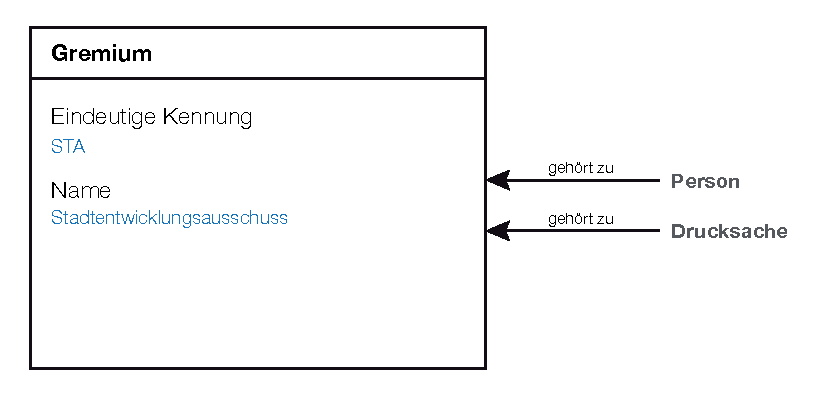
\includegraphics{images/datenmodell_gremium.png}
\caption{Objekttyp Committee}
\end{figure}

\subsubsection{Eigenschaften}

\begin{description}
\item[Schlüssel (\texttt{id})]
Zur eindeutigen Identifizierung des Gremiums im Kontext einer bestimmten
Körperschaft. In der Praxis kommen sowohl numerische IDs als auch
Namenskürzel (Beispiel: ``STA'' für den Stadtentwicklungsausschuss) vor.
Beides sollte hier Verwendung finden können.
\item[Name (\texttt{name})]
Der Name des Gremiums. Beispiele: ``Rat'', ``Hauptausschuss'',
``Bezirksvertretung 1 (Innenstadt)''
\item[Kurzname (\texttt{short\_name})]
\emph{Optional}. Eine zur Anzeige bestimmte, kürzere Form des Namens.
\item[Zuletzt geändert (\texttt{last\_modified})]
Datum und Uhrzeit der letzten Änderung
\end{description}

\subsubsection{Beziehungen}

\begin{itemize}
\item
  Objekte vom Typ \texttt{oparl:Person} referenzieren auf Gremien, um
  die Mitgliedschaft/Zugehörigkeit einer Person im/zum Gremium zu
  kennzeichnen. Diese Beziehung ist datiert. Das bedeutet, sie hat einen
  Anfangszeitpunkt und ggf. einen Endzeitpunkt.
\item
  Objekte vom Typ ``Drucksache'' verweisen auf Gremien. Beispielsweise
  wird eine Anfrage oder ein Antrag dem Rat und/oder einer bestimmten
  Bezirksvertretung zugeordnet. Details zu dieser Beziehung werden unter
  ``Drucksache'' erläutert.
\item
  Das Gremium verweist auf die Körperschaft, zu der das Gremium gehört.
\end{itemize}

\subsubsection{Beispiel}

\begin{Shaded}
\begin{Highlighting}[]
\NormalTok{\{}
    \DataTypeTok{"id"}\NormalTok{: }\StringTok{"7"}\NormalTok{,}
    \DataTypeTok{"name"}\NormalTok{: }\StringTok{"Finanzausschuss"}\NormalTok{,}
    \DataTypeTok{"short_name"}\NormalTok{: }\StringTok{"FA"}\NormalTok{,}
    \DataTypeTok{"body"}\NormalTok{: }\StringTok{"1"}\NormalTok{,}
    \DataTypeTok{"last_modified"}\NormalTok{: }\StringTok{"2012-08-16T14:05:27+02:00"}
\NormalTok{\}}
\end{Highlighting}
\end{Shaded}

\subsection{oparl:Person (Person)}

Jede natürliche Person, die Mitglied eines Gremiums ist, ist als
\texttt{oparl:Person} im Datenmodell eindeutig identifizierbar.

\begin{figure}[htbp]
\centering
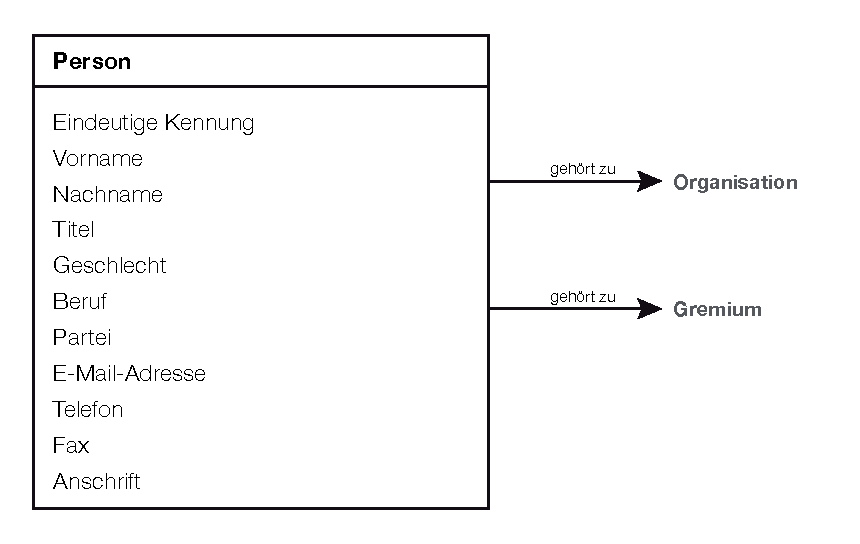
\includegraphics{images/datenmodell_person.png}
\caption{Objekttyp Person}
\end{figure}

\subsubsection{Eigenschaften}

\begin{description}
\item[Schlüssel (\texttt{id})]
Zur eindeutigen Identifizierung sollte jede Person eine Kennung
besitzen, die keinen Änderungen unterworfen ist und aus diesem Grund
nicht mit dem Namen in Verbindung stehen sollte. Viele RIS nutzen rein
numerische Kennungen.
\item[Vorname (\texttt{first\_name})]
Der Vorname der Person.
\item[Nachname (\texttt{last\_name})]
Der Nachname der Person.
\item[Titel (\texttt{academic\_title})]
\emph{Optional}. Akademische Titel wie ``Dr.'' und ``Prof.~Dr.''
\item[Geschlecht (\texttt{sex})]
\emph{Optional}. Weiblich (Wert \texttt{F} für \emph{female}), männlich
(Wert \texttt{M} für \emph{male}), anderes (Wert \texttt{O} für
\emph{others})
\item[Beruf (\texttt{profession})]
\emph{Optional}. Z.B. ``Rechtsanwalt''
\item[E-Mail-Adresse (\texttt{email})]
\emph{Optional}.
\item[Telefon (\texttt{phone})]
\emph{Optional}.
\item[Fax (\texttt{fax})]
\emph{Optional}.
\item[Anschrift (\texttt{address})]
\emph{Optional}. Straße und Hausnummer, Postleitzahl und Ort
\item[Zuletzt geändert (\texttt{last\_modified})]
Datum und Uhrzeit der letzten Änderung
\end{description}

\paragraph{Anmerkungen}

\begin{itemize}
\item
  Das System von Euskirchen scheint Vor- und Nachname (evtl. einschl.
  Titel) in einem gemeinsamen Feld ``Name'' zu führen. Ob das System
  hier technisch differenziert, ist unklar. Falls einzelne Systeme den
  angezeigten Namen nur als ganzes speichern, sollte dies für den
  Standard übernommen werden, da es für die meisten Anwendungen
  ausreichen sollte.
\item
  Das System PROVOX unterscheidet zwischen privaten und geschäftlichen
  Anschriften.
\end{itemize}

\subsubsection{Beziehungen}

\begin{itemize}
\item
  Objekte vom Typ \texttt{oparl:Person} können einer Organisation, z.B.
  einer Fraktion, zugeornet werden. Diese Beziehung ist datiert.
\item
  Objekte vom Typ \texttt{oparl:Person} können einem oder mehreren
  Gremien zugewiesen werden, um die Mitgliedschaft in diesem Gremium
  darzustellen. Diese Beziehungen sind ebenfalls datiert.
\end{itemize}

\subsubsection{Beispiel}

\begin{Shaded}
\begin{Highlighting}[]
\NormalTok{\{}
    \DataTypeTok{"id"}\NormalTok{: }\StringTok{"1000"}\NormalTok{,}
    \DataTypeTok{"first_name"}\NormalTok{: }\StringTok{"Max"}\NormalTok{,}
    \DataTypeTok{"last_name"}\NormalTok{: }\StringTok{"Mustermann"}\NormalTok{,}
    \DataTypeTok{"academic_title"}\NormalTok{: }\StringTok{"Dr."}\NormalTok{,}
    \DataTypeTok{"sex"}\NormalTok{: }\StringTok{"M"}\NormalTok{,}
    \DataTypeTok{"profession"}\NormalTok{: }\StringTok{"Rechtsanwalt"}\NormalTok{,}
    \DataTypeTok{"email"}\NormalTok{: }\StringTok{"max@mustermann.de"}\NormalTok{,}
    \DataTypeTok{"phone"}\NormalTok{: }\StringTok{"+4977777"}\NormalTok{,}
    \DataTypeTok{"fax"}\NormalTok{: }\StringTok{"+4988888"}\NormalTok{,}
    \DataTypeTok{"address"}\NormalTok{: }\StringTok{"Musterstraße 5, 11111 Musterort"}\NormalTok{,}
    \DataTypeTok{"last_modified"}\NormalTok{: }\StringTok{"2012-08-16T14:05:27+02:00"}\NormalTok{,}
    \DataTypeTok{"organisations"}\NormalTok{: [}
        \NormalTok{\{}
            \DataTypeTok{"id"}\NormalTok{: }\StringTok{"2000"}\NormalTok{,}
            \DataTypeTok{"start"}\NormalTok{: }\StringTok{"2011-03-01"}\NormalTok{,}
            \DataTypeTok{"end"}\NormalTok{: }\StringTok{"2013-02-28"}
        \NormalTok{\},}
        \NormalTok{\{}
            \DataTypeTok{"id"}\NormalTok{: }\StringTok{"2001"}\NormalTok{,}
            \DataTypeTok{"start"}\NormalTok{: }\StringTok{"2013-03-01"}
        \NormalTok{\}}
    \NormalTok{],}
    \DataTypeTok{"committees"}\NormalTok{: [}
        \NormalTok{\{}
            \DataTypeTok{"id"}\NormalTok{: }\StringTok{"7"}\NormalTok{,}
            \DataTypeTok{"start"}\NormalTok{: }\StringTok{"2013-01-01"}
        \NormalTok{\}}
    \NormalTok{]}
\NormalTok{\}}
\end{Highlighting}
\end{Shaded}

\subsection{oparl:Organization (Organisation)}

Organisationen sind üblicherweise Parteien bzw. Fraktionen, denen die
Personen angehören können.

\begin{figure}[htbp]
\centering
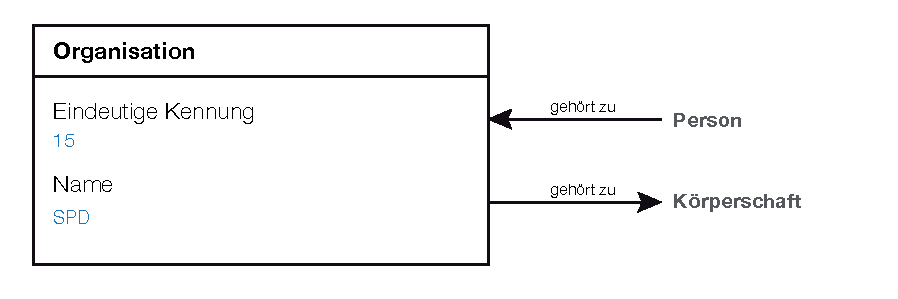
\includegraphics{images/datenmodell_organisation.png}
\caption{Objekttyp Organisation}
\end{figure}

\subsubsection{Eigenschaften}

\begin{description}
\item[Schlüssel (\texttt{id})]
Zur eindeutigen Kennzeichnung einer Organisation innerhalb des Systems
\item[Name (\texttt{name})]
Der gebräuchliche Name der Organisation, z.B. ``SPD'' oder ``DIE
LINKE''.
\item[Zuletzt geändert (\texttt{last\_modified})]
Datum und Uhrzeit der letzten Änderung
\end{description}

\paragraph{Anmerkungen}

\begin{itemize}
\item
  Unklar ist bislang, ob Organisationen in der Praxis eher Fraktionen
  (``SPD-Fraktion im Kölner Rat'', ``SPD-Fraktion in Köln-Innenstadt'')
  abbilden oder ob eher Ortsverbände von Parteien (``SPD Köln'') gemeint
  sein werden. Einblicke, wie gängige Systeme dies handhaben, sollten
  evtl. gesammelt und berücksichtigt werden.
\item
  Es wird die Schreibweise ``Organization'' (und nicht ``Organisation'')
  verwendet, da diese in allen englischen Sprachräumen problemlos
  verwendet werden kann. Siehe dazu Abschnitt 3, Fussnote 1 auf dieser
  Seite: http://popoloproject.com/specs/organization.html
\end{itemize}

\subsubsection{Beziehungen}

\begin{itemize}
\item
  Jede \texttt{oparl:Organization} gehört zu einer Körperschaft.
\item
  Personen können Organisationen angehören (\emph{datiert}).
\end{itemize}

\subsubsection{Beispiel}

\begin{Shaded}
\begin{Highlighting}[]
\NormalTok{\{}
    \DataTypeTok{"id"}\NormalTok{: }\StringTok{"15"}\NormalTok{,}
    \DataTypeTok{"name"}\NormalTok{: }\StringTok{"SPD"}\NormalTok{,}
    \DataTypeTok{"body"}\NormalTok{: }\StringTok{"1"}\NormalTok{,}
    \DataTypeTok{"last_modified"}\NormalTok{: }\StringTok{"2012-08-16T14:05:27+02:00"}
\NormalTok{\}}
\end{Highlighting}
\end{Shaded}

\subsection{oparl:Meeting (Sitzung)}

Eine Sitzung ist die Versammlung der Mitglieder eines Gremiums oder
mehrerer Gremien zu einem bestimmten Zeitpunkt an einem bestimmten Ort.

Die geladenen Teilnehmer der Sitzung sind jeweils als „Person`` in
entsprechender Form referenziert. Verschiedene Dokumente (Einladung,
Ergebnis- und Wortprotokoll, sonstige Anlagen) können referenziert
werden.

\begin{figure}[htbp]
\centering
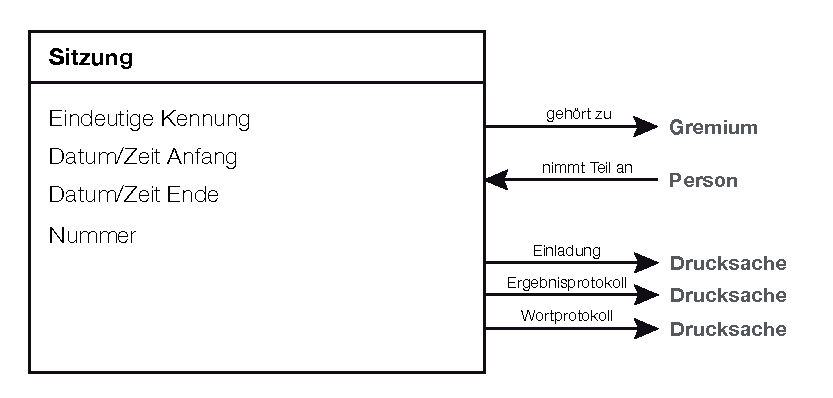
\includegraphics{images/datenmodell_sitzung.png}
\caption{Objekttyp Meeting}
\end{figure}

\subsubsection{Eigenschaften}

\begin{description}
\item[Schlüssel (\texttt{id})]
Zur eindeutigen Identifizierung der Sitzung innerhalb des Systems. In
der Praxis wird ein solcher Schlüssel entweder durch eine numerische ID
gebildet oder durch Kombination mehrerer Merkmale wie dem Kürzel des
Gremiums, der laufenden Nummer der Sitzung in einem Jahr und der
Jahreszahl (z.B. ``BV1/0034/2012'').
\item[Nummer (\texttt{sequence\_number})]
\emph{Optional}. Laufende Nummer der Sitzung, üblicherweise innerhalb
der Wahlperiode mit 1 beginnend. In der Praxis wird dadurch z.B. die
``2. Sitzung des Rats'' gekennzeichnet. Ist dieses Feld gesetzt, MUSS
ein numerischer Wert enthalten sein.
\item[Anfang (\texttt{start})]
Datum und ggf. Uhrzeit des Anfangszeitpunkts der Sitzung
\item[Ende (\texttt{end})]
\emph{Optional}. Datum und Uhrzeit vom Ende der Sitzung
\item[Ort (\texttt{address})]
\emph{Optional}. Textliche Information zum Ort der Sitzung, z.B.
``Rathaus, Raum 136''.
\item[Zuletzt geändert (\texttt{last\_modified})]
Datum und Uhrzeit der letzten Änderung
\end{description}

\subsubsection{Beziehungen}

\begin{itemize}
\item
  Sitzungen sind mindestens einem Gremium zugeordnet
\item
  Einer Sitzung sind Personen zugeordnet, um die Teilnahme an der
  Sitzung auszudrücken.
\item
  Dokumente können vom Typ \texttt{oparl:Meeting} \emph{optional} zu
  mehreren Zwecken referenziert werden:

  \begin{itemize}
  \item
    Zum Verweis auf die Einladung zur Sitzung
  \item
    Zum Verweis auf das Ergebnisprotokoll zur Sitzung
  \item
    Zum Verweis auf das Wortprotokoll zur Sitzung
  \end{itemize}
\item
  Weiterhin können Sitzungen beliebige weitere Dokumente, die keine
  eigenständigen Drucksachen sind, referenzieren. Dabei handelt es sich
  dann um nicht weiter spezifizierte Anlagen.
\end{itemize}

\subsubsection{Beispiel}

\begin{Shaded}
\begin{Highlighting}[]
\NormalTok{\{}
    \DataTypeTok{"id"}\NormalTok{: }\StringTok{"3271"}\NormalTok{,}
    \DataTypeTok{"identifier"}\NormalTok{: }\StringTok{"STA/0034/2012"}\NormalTok{,}
    \DataTypeTok{"start"}\NormalTok{: }\StringTok{"2013-01-04T08:00:00+01:00"}\NormalTok{,}
    \DataTypeTok{"end"}\NormalTok{: }\StringTok{"2013-01-04T12:00:00+01:00"}\NormalTok{,}
    \DataTypeTok{"address"}\NormalTok{: }\StringTok{"Rathaus, Raum 136"}\NormalTok{,}
    \DataTypeTok{"sequence_number"}\NormalTok{: }\DecValTok{1}\NormalTok{,}
    \DataTypeTok{"committees"}\NormalTok{: [}\StringTok{"STA"}\NormalTok{],}
    \DataTypeTok{"people"}\NormalTok{: [}\StringTok{"1000"}\NormalTok{, }\StringTok{"1001"}\NormalTok{],}
    \DataTypeTok{"invitation"}\NormalTok{: }\StringTok{"0001/2013"}\NormalTok{,}
    \DataTypeTok{"result_minutes"}\NormalTok{: }\StringTok{"0002/2013"}\NormalTok{,}
    \DataTypeTok{"verbatim_minutes"}\NormalTok{: }\StringTok{"0003/2013"}\NormalTok{,}
    \DataTypeTok{"attachments"}\NormalTok{: [}
        \StringTok{"0004/2013"}\NormalTok{,}
        \StringTok{"0005/2013"}
    \NormalTok{],}
    \DataTypeTok{"last_modified"}\NormalTok{: }\StringTok{"2012-01-08T14:05:27+01:00"}
\NormalTok{\}}
\end{Highlighting}
\end{Shaded}

\subsection{oparl:AgendaItem (Tagesordnungspunkt)}

Der Tagesordnungspunkt wird für eine bestimmte Sitzung angelegt, erhält
eine (innerhalb dieser Sitzung eindeutige) Nummer und einen Titel
(Betreff). Nach der Sitzung wird dem Tagesordnungspunkt außerdem ein
Ergebnis angehängt. Unter Umständen kann dem Tagesordnungspunkt ein
bestimmter Beschlusstext beigefügt sein.

Überlicherweise haben Sitzungen mehrere Tagesordnungspunkte.

\begin{figure}[htbp]
\centering
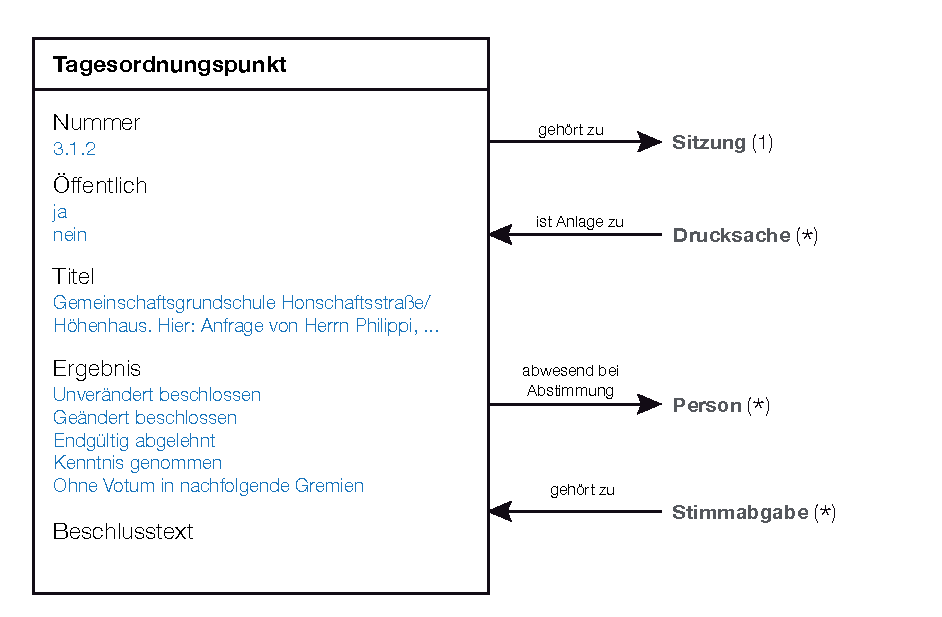
\includegraphics{images/datenmodell_tagesordnungspunkt.png}
\caption{Objekttyp AgendaItem}
\end{figure}

\subsubsection{Eigenschaften}

\begin{description}
\item[Nummer (\texttt{identifier})]
Beispiel: ``1.2.3''. Diese Nummer gibt an, in welcher Reihenfolge die
Tagesordnungspunkte einer Sitzung normalerweise behandelt werden. Im
Kontext einer Sitzung ist diese Nummer eindeutig.
\item[Öffentlich (\texttt{public})]
Kennzeichnet, ob der Tagesordnungspunkt in öffentlicher Sitzung
behandelt wird. Kann die Werte \texttt{true} (öffentlich) oder
\texttt{false} annehmen.
\item[Titel (\texttt{title})]
Das Thema des Tagesordnungspunktes
\item[Ergebnis (\texttt{result})]
\emph{Optional}. Kategorische Information darüber, welches Ergebnis die
Beratung des Tagesordnungspunktes gebracht hat. In der Praxis sind hier
Kategorien wie ``Unverändert beschlossen'', ``Geändert beschlossen'',
``Endgültig abgelehnt'', ``Zur Kenntnis genommen'', ``Ohne Votum in
nachfolgende Gremien überwiesen'' und weitere zu erwarten.
\item[Ergebnis Details (\texttt{result\_details})]
\emph{Optional}. Ermöglicht die Angabe zusätzlicher Textinformationen
zum Ergebnis, zum Beispiel im Fall der Verweisung an ein anderes Gremium
die Angabe, an welches Gremium verwiesen wurde.
\item[Beschlusstext (\texttt{resolution\_text})]
\emph{Optional}. Falls in diesem Tagesordnungspunkt ein Beschluss
gefasst wurde, kann der Text hier hinterlegt werden. Das ist besonders
dann in der Praxis relevant, wenn der gefasste Beschluss (z.B. durch
Änderungsantrag) von der Beschlussvorlage abweicht.
\item[Zuletzt geändert (\texttt{last\_modified})]
Datum und Uhrzeit der letzten Änderung
\end{description}

\paragraph{Anmerkungen}

\begin{itemize}
\item
  Einige Systeme vergeben zu Tagesordnungspunkten intern
  unveränderliche, numerische IDs. Es ist unklar, ob es zusätzlichen
  Nutzen bringt, derartige IDs, neben den Nummern, in den Standard zu
  übernehmen. Dies würde vermutlich nur Sinn ergeben, wenn es als
  Pflichtfeld gelten könnte.
\item
  Teil der Beratungen über einheitliche Nomenklatur im Standard sollte
  sein, eine Vereinheitlichung der Werte für die Eigenschaft
  \texttt{result} zu diskutieren.
\end{itemize}

\subsubsection{Beziehungen}

\begin{itemize}
\item
  Jeder Tagesordnungspunkt gehört zu genau einem \texttt{oparl:Meeting}.
\item
  Der Tagesordnungspunkt kann auf eine Drucksache verweisen, die im
  Rahmen dieses Tagesordnungspunkt beraten werden soll.
\item
  Es können \texttt{oparl:Person} Objekte referenziert werden, die
  während der Abstimmung zu diesem Tagesordnungspunkt \emph{nicht}
  anwesend waren.
\end{itemize}

\subsubsection{Beispiel}

\begin{Shaded}
\begin{Highlighting}[]
\NormalTok{\{}
    \DataTypeTok{"meeting"}\NormalTok{: }\StringTok{"3271"}\NormalTok{,}
    \DataTypeTok{"identifier"}\NormalTok{: }\StringTok{"3.1.2"}\NormalTok{,}
    \DataTypeTok{"public"}\NormalTok{: }\DecValTok{true}\NormalTok{,}
    \DataTypeTok{"title"}\NormalTok{: }\StringTok{"Gemeinschaftsgrundschule Hornschaftsstraße/Höhenhaus. Hier: Anfrage von Herrn Philippi"}\NormalTok{,}
    \DataTypeTok{"result"}\NormalTok{: }\StringTok{"Geändert beschlossen"}\NormalTok{,}
    \DataTypeTok{"resolution_text"}\NormalTok{: }\StringTok{"Der Beschluss weicht wie folgt vom Antrag ab: ..."}\NormalTok{,}
    \DataTypeTok{"people_absent"}\NormalTok{: [}\StringTok{"1002"}\NormalTok{, }\StringTok{"1003"}\NormalTok{],}
    \DataTypeTok{"last_modified"}\NormalTok{: }\StringTok{"2012-08-16T14:05:27+02:00"}
\NormalTok{\}}
\end{Highlighting}
\end{Shaded}

\subsection{oparl:Paper (Drucksache)}

Eine Drucksache bildet Mitteilungen, Antworten auf Anfragen,
Beschlussvorlagen, Anfragen, Anträge und weitere Vorlagen ab. Jede
Drucksache erhält eine eindeutige Kennung.

Die Drucksache hat im Informationsmodell eine hervorgehobene Bedeutung.
Im Fall eines Antrags kann mit einer einzigen Drucksache ein über Monate
oder Jahre dauernder politischer Entscheidungsprozess verbunden sein. In
dem Zusammenhang entstehen üblicherweise weitere Drucksachen.

Drucksachen spielen in der schriftlichen wie mündlichen Kommunikation
eine besondere Rolle, da in vielen Texten auf bestimmte Drucksachen
Bezug genommen wird. Hierbei kommen in Ratsinformationssystemen
unveränderliche Kennungen der Drucksachen zum Einsatz.

\begin{figure}[htbp]
\centering
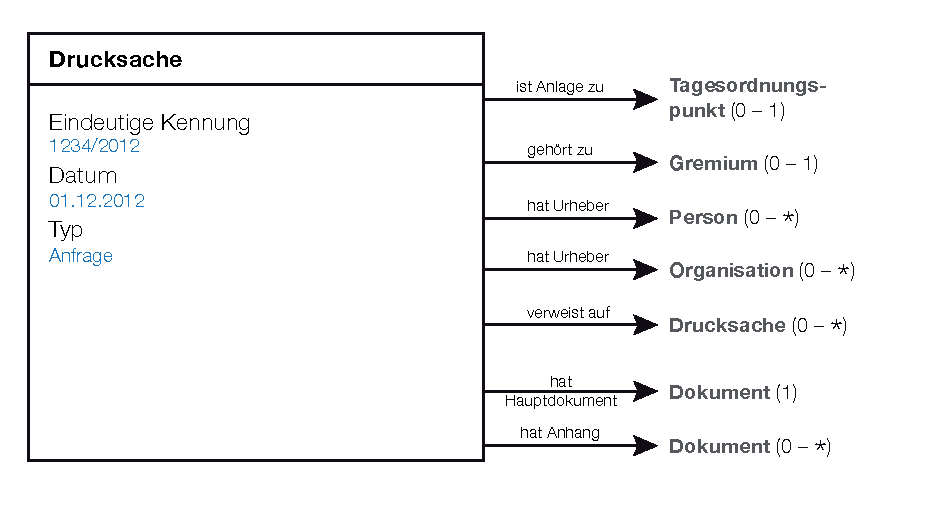
\includegraphics{images/datenmodell_drucksache.png}
\caption{Objekttyp Paper}
\end{figure}

Jede Drucksache ist über die Eigenschaft ``Typ'' als eine der folgenden
Arten von Drucksachen gekennzeichnet:

\begin{itemize}
\item
  \textbf{Beschlussvorlage}: Entscheidungsvorschlag der Verwaltung
\item
  \textbf{Antrag}: Entscheidungsvorschlag einer Fraktionen bzw. mehrerer
  Fraktionen oder einer/mehrerer Einzelperson/en
\item
  \textbf{Anfrage}: Frage(n) einer oder mehrerer Fraktion oder
  Einzelpersonen an die Verwaltung
\item
  \textbf{Mitteilung/Stellungnahme der Verwaltung}: Eine Information der
  Verwaltung an einzelne oder mehrere Gremien. Darunter fallen nicht
  Beantwortungen von Anfragen.
\item
  \textbf{Beantwortung einer Anfrage}: Antwort der Verwaltung auf
  (mündliche oder schriftliche) Anfragen
\end{itemize}

\subsubsection{Eigenschaften}

\begin{description}
\item[Schlüssel (\texttt{id})]
Die Kennung einer Drucksache muss für die jeweilige Körperschaft
eindeutig sein. Sie kann sowohl Ziffern als auch Buchstaben enthalten.
Einige Systeme (z.B. Köln) verwenden besondere Trennzeichen wie ``/'',
um eine Jahreszahl von einer laufenden Nummer abzutrennen. Weiterhin
werden mancherorts führende Nullen verwendet.
\item[Datum (\texttt{date})]
Datum der Veröffentlichung
\item[Typ (\texttt{type})]
Art der Drucksache (Erläuterung siehe oben)
\item[Zuletzt geändert (\texttt{last\_modified})]
Datum und Uhrzeit der letzten Änderung
\end{description}

\subsubsection{Beziehungen}

\begin{itemize}
\item
  Es muss genau ein \textbf{Hauptdokument} (\texttt{oparl:Document})
  referenziert werden.
\item
  Es können beliebig viele weitere Dokumente referenziert werden, die
  als nachgeordnete \textbf{Anlagen} zur Drucksache verstanden werden.
\item
  Die Drucksache ist beliebig vielen Gremien zuzuordnen, in denen diese
  beraten wird.
\item
  Drucksachen können \textbf{Urhebern} zugewiesen werden. Im Fall von
  Mitteilungen der Verwaltung ist dies oft der Oberbürgermeister. Bei
  Anträgen oder Anfragen können Organisationen oder Einzelpersonen
  referenziert werden. Es können stets mehrere Uhrheber verknüpft
  werden.
\item
  Es können beliebig viele \textbf{Orte} (siehe Objekttyp ``Ort'')
  referenziert werden, die im Inhalt der Drucksache behandelt werden.
  Beispiel: Beschlussvorlage zur Freigabe von Mitteln für die Sanierung
  eines Sportplatzes, wobei der Ort die Lage des Sportplatzes genau
  beschreibt. (TODO)
\item
  Drucksachen können auf andere Drucksachen referenzieren. Diese
  Verweise können verschiedene semantische Beziehungen ausdrücken. So
  kann eine Drucksache auf eine übergeordnete oder eine oder mehrere
  untergeordnete Drucksachen verweisen. Beim Drucksachen-Typ
  ``Beantwortung einer Anfrage'' ist die Drucksache zu referenzieren,
  die die ursprüngliche \textbf{Anfrage} beinhaltet. Denkbar sind auch
  Verweise auf frühere Drucksachen zum selben Thema. Zu klären ist, wie
  die verschiedenen möglichen Beziehungen formell ausgedrückt werden.
\item
  Drucksachen können zu beliebig vielen Tagesordnungspunkten in
  Beziehung stehen, um die \textbf{Beratungsfolge} einer Drucksache
  abzubilden. Hierbei kann die Beziehung jeweils mit einer Zuständigkeit
  versehen sein, die noch näher zu bestimmen ist (TODO).
\end{itemize}

\subsubsection{Beispiel}

\begin{Shaded}
\begin{Highlighting}[]
\NormalTok{\{}
    \DataTypeTok{"id"}\NormalTok{: }\StringTok{"1234/2012"}\NormalTok{,}
    \DataTypeTok{"date"}\NormalTok{: }\StringTok{"2013-01-04"}\NormalTok{,}
    \DataTypeTok{"type"}\NormalTok{: }\StringTok{"Beantwortung einer Anfrage"}\NormalTok{,}
    \DataTypeTok{"related_papers"}\NormalTok{: [}
        \StringTok{"0768/2012"}
    \NormalTok{],}
    \DataTypeTok{"main_document"}\NormalTok{: }\StringTok{"3000.pdf"}\NormalTok{,}
    \DataTypeTok{"attachments"}\NormalTok{: [}
        \StringTok{"3002.pdf"}\NormalTok{,}
        \StringTok{"3003.pdf"}
    \NormalTok{],}
    \DataTypeTok{"locations"}\NormalTok{: [}
        \NormalTok{\{}
            \DataTypeTok{"description"}\NormalTok{: }\StringTok{"Theodor-Heuss-Ring 1"}\NormalTok{,}
            \DataTypeTok{"lat"}\NormalTok{: }\FloatTok{7.148}\NormalTok{,}
            \DataTypeTok{"lon"}\NormalTok{: }\FloatTok{50.023}
        \NormalTok{\}}
    \NormalTok{],}
    \DataTypeTok{"committees"}\NormalTok{: [}\StringTok{"STA"}\NormalTok{],}
    \DataTypeTok{"creators"}\NormalTok{: [}
        \NormalTok{\{}
            \DataTypeTok{"typ"}\NormalTok{: }\StringTok{"Organisation"}\NormalTok{,}
            \DataTypeTok{"id"}\NormalTok{: }\StringTok{"2000"}
        \NormalTok{\},}
        \NormalTok{\{}
            \DataTypeTok{"typ"}\NormalTok{: }\StringTok{"Person"}\NormalTok{,}
            \DataTypeTok{"id"}\NormalTok{: }\StringTok{"1000"}
        \NormalTok{\}}
    \NormalTok{],}
    \DataTypeTok{"consultations"}\NormalTok{: [}
        \NormalTok{\{}
            \DataTypeTok{"meeting"}\NormalTok{: }\StringTok{"3271"}\NormalTok{,}
            \DataTypeTok{"agendaitem"}\NormalTok{: }\StringTok{"3.1.2"}\NormalTok{,}
            \DataTypeTok{"role"}\NormalTok{: }\StringTok{"Federführende Beratung"}
        \NormalTok{\}}
    \NormalTok{],}
    \DataTypeTok{"last_modified"}\NormalTok{: }\StringTok{"2013-01-08T12:05:27+01:00"}
\NormalTok{\}}
\end{Highlighting}
\end{Shaded}

\subsection{oparl:Document (Dokument)}

Ein Dokument hält Metadaten einer Datei vor, beispielsweise einer
PDF-Datei, eines RTF- oder ODF-Dokuments (oder auch einer Datei in einem
proprietären Format).

Wird von einem Dokument in einem Nicht-PDF-Format (z.B. RTF oder ODF)
eine PDF-Ableitung hinterlegt, ist diese Ableitung ebenfalls ein
Dokument. Um zu zeigen, dass es sich um eine Ableitung handelt, verweist
dieses auf das Original als ``Master''.

Im Unterschied zur Drucksache benötigt das Dokument keine
nutzerfreundliche Kennung.

\begin{figure}[htbp]
\centering
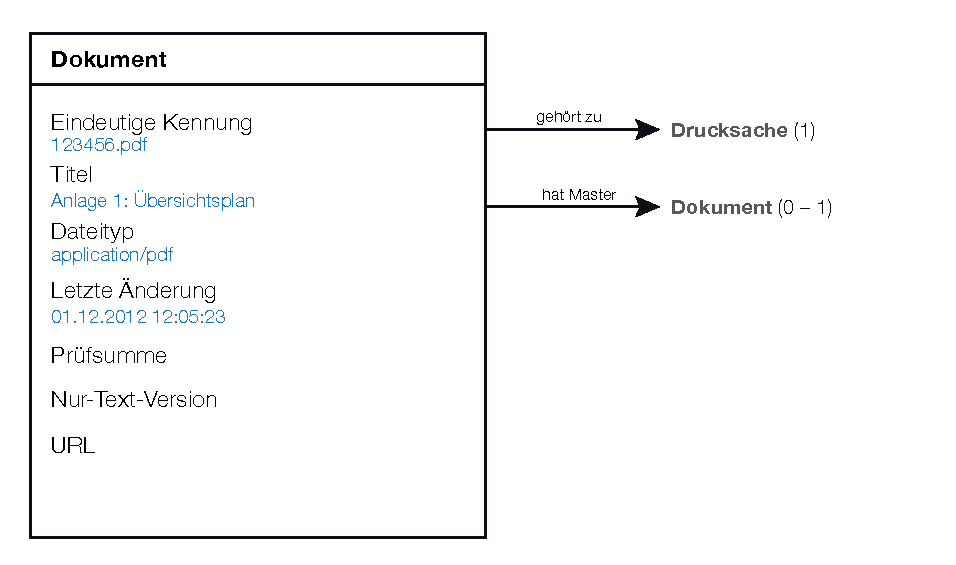
\includegraphics{images/datenmodell_dokument.png}
\caption{Objekttyp Document}
\end{figure}

\subsubsection{Eigenschaften}

\begin{description}
\item[Schlüssel (\texttt{id})]
Unveränderliche Kennung
\item[Name (\texttt{name})]
Dateiname, z.B. ``12345.pdf''
\item[Dateityp (\texttt{mime\_type})]
Mime-Typ des Inhalts, z.B. ``application/pdf''
\item[Veröffentlichungsdatum (\texttt{date})]
Datum des Tages, an dem das Dokument ins System eingestellt wurde
\item[Änderungsdatum und -uhrzeit (\texttt{last\_modified})]
Datum und Uhrzeit der letzten Änderung des Dokuments
\item[Prüfsumme (\texttt{sha1\_checksum})]
SHA1-Prüfsumme des Dokumenteninhalts
\item[URL (\texttt{url})]
URL zum Abruf der Daten dieses Dokuments mittels HTTP GET-Aufruf
\item[Nur-Text-Version (\texttt{text})]
Reine Text-Wiedergabe des Dokumenteninhalts, sofern es sich nicht um
eine reine Abbildung handelt.
\end{description}

\subsubsection{Beziehungen}

\begin{itemize}
\item
  Dokumente gehören zwingend zu einer \textbf{Drucksache}, optional auch
  zu mehreren. Ein Dokument kann entweder als Hauptdokument einer
  Drucksache oder als Anlage eingestuft sein.
\item
  Ein Dokument kann auf ein anderes Dokument referenzieren, wenn es von
  dem anderen Dokument abstammt. So ist es möglich, von einem
  abgeleiteten Dokument zu seinem Dokumenten-Master zu gelangen
  (Beispiel: von einem PDF-Dokument zum OpenOffice-Original).
\end{itemize}

\begin{Shaded}
\begin{Highlighting}[]
\NormalTok{\{}
    \DataTypeTok{"id"}\NormalTok{: }\StringTok{"3000"}\NormalTok{,}
    \DataTypeTok{"name"}\NormalTok{: }\StringTok{"3000.pdf"}\NormalTok{,}
    \DataTypeTok{"mime_type"}\NormalTok{: }\StringTok{"application/pdf"}\NormalTok{,}
    \DataTypeTok{"date"}\NormalTok{: }\StringTok{"2013-01-04T07:54:13+01:00"}\NormalTok{,}
    \DataTypeTok{"last_modified"}\NormalTok{: }\StringTok{"2013-01-04T07:54:13+01:00"}\NormalTok{,}
    \DataTypeTok{"sha1_checksum"}\NormalTok{: }\StringTok{"da39a3ee5e6b4b0d3255bfef95601890afd80709"}\NormalTok{,}
    \DataTypeTok{"url"}\NormalTok{: }\StringTok{"http://ris.beispielstadt.de/api/documents/3000.pdf"}\NormalTok{,}
    \DataTypeTok{"text"}\NormalTok{: }\StringTok{"Der Übersichtsplan zeigt alle Ebenen des ..."}\NormalTok{,}
    \DataTypeTok{"master"}\NormalTok{: }\StringTok{"2099"}
\NormalTok{\}}
\end{Highlighting}
\end{Shaded}

\subsection{oparl:Consultation (Beratung)}

\subsection{oparl:Location (Ort)}

Dieser Objekttyp dient dazu, einen Ortsbezug einer Drucksache formal
abzubilden. Ortsangaben können sowohl aus Textinformationen bestehen
(beispielsweise der Name einer Straße/eines Platzes oder eine genaue
Adresse) als auch aus Geodaten.

OParl sieht die Angabe von Geodaten in Anlehnung an die
GeoJSON-Spezifikation {[}13{]} vor. Die GeoJSON-Spezifikation erlaubt
die Abbildung von vielen unterschiedlichen Geometrien wie Punkten,
Pfaden und Polygonen. Während GeoJSON zu jedem Geodaten-Objekt auch die
Speicherung zusätzlicher Metadaten ermöglicht, beschränkt sich OParl
ledliglich auf das \texttt{geometry}-Attribut in GeoJSON. Sämtliche
Geo-Koordinatenangaben werden in in OParl im WGS-84-System {[}11{]}
erwartet.

\begin{figure}[htbp]
\centering
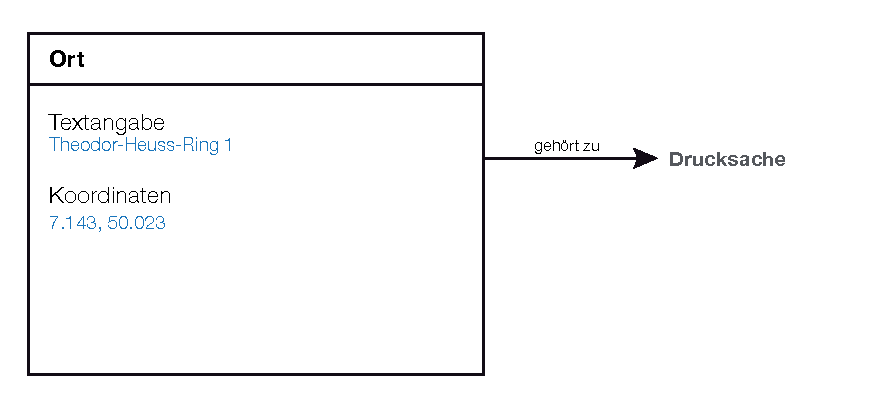
\includegraphics{images/datenmodell_ort.png}
\caption{Objekttyp Location}
\end{figure}

\subsubsection{Eigenschaften}

\begin{description}
\item[Textanabe (\texttt{description})]
\emph{Optional.} Textliche Beschreibung eines Orts, z.B. in Form einer
Adresse
\item[Koordinaten (\texttt{geometry})]
\emph{Optional.} GeoJSON geometry Objekt
\item[Zuletzt geändert (\texttt{last\_modified})]
Datum und Uhrzeit der letzten Änderung
\end{description}

\subsubsection{Beziehungen}

\begin{itemize}
\item
  Orte können mit Drucksachen in Verbindung stehen.
\end{itemize}

\begin{Shaded}
\begin{Highlighting}[]
\NormalTok{\{}
    \DataTypeTok{"description"}\NormalTok{: }\StringTok{"Honschaftsstraße 312, 51061 Köln"}\NormalTok{,}
    \DataTypeTok{"geometry"}\NormalTok{: \{}
        \DataTypeTok{"type"}\NormalTok{: }\StringTok{"Point"}\NormalTok{,}
        \DataTypeTok{"coordinates"}\NormalTok{: [}\FloatTok{7.03291}\NormalTok{, }\FloatTok{50.98249}\NormalTok{]}
    \NormalTok{\},}
    \DataTypeTok{"last_modified"}\NormalTok{: }\StringTok{"2013-02-14T14:05:27+01:00"}
\NormalTok{\}}
\end{Highlighting}
\end{Shaded}

\subsection{oparl:Contact (Kontakt)}

\section{Fußnoten}

{[}11{]}: World Geodetic System 1984 (EPSG:4326), wird unter anderem
auch vom Global Positioning System (GPS) verwendet.

{[}13{]}: GeoJSON \href{http://www.geojson.org/}{www.geojson.org}

{[}14{]}: Frankfurt Gestalten
\href{http://www.geojson.org/}{www.geojson.org}

{[}15{]}: Offenes Köln \href{http://offeneskoeln.de/}{offeneskoeln.de}

{[}16{]}: OpenRuhr:RIS
\href{http://openruhr.de/openruhrris/}{openruhr.de/openruhrris}

\section{Glossar}

\begin{description}
\item[JSON-LD]
JSON for Linked Data
\item[RIS]
Ratsinformationssystem
\item[WGS 84]
World Geodetic System 1984. Ein weltweites Referenzsystem für die
Interpretation von Geokoordinaten-Angaben.
\end{description}

\end{document}
